\documentclass[12pt,a4paper,twoside,openright]{report}


\usepackage{graphics}       % Graphics commands
\usepackage{wrapfig}        % Wrapping text around figures
\usepackage{epsfig}         % Embed encapsulated postscript
\usepackage{rotating}       % Extra graphics rotation
\usepackage{longtable}      % Page breaks within tables
\usepackage{supertabular}   % Page breaks within tables
\usepackage{multicol}       % Allows table cells to span cols
\usepackage{multirow}       % Allows table cells to span rows
\usepackage{texnames}       % Macros for common tex names

\usepackage{listings}       % Source code listings
\usepackage{array}          % Array environment
\usepackage{url}            % URL formatting
\usepackage{amsmath}        % American Mathematical Society
\usepackage{amssymb}        % Maths symbols
\usepackage{amsthm}         % Theorems
%\usepackage{mathpartir}     % Proofs and inference rules
\usepackage{verbatim}       % Verbatim blocks
\usepackage{ifthen}         % Conditional processing in tex
\usepackage{xcolor}         % X11 colour names
\usepackage{ulem}

\usepackage{tikz}
\usetikzlibrary{arrows, automata}
\usepackage[margin=25mm]{geometry}
\usetikzlibrary{shapes,fit,calc,positioning}

\usepackage{float}

\usepackage{biblatex}
\addbibresource{dissertation.bib}

\usepackage{pgfplots, pgfplotstable}
\pgfplotsset{compat=1.12}

\usepackage[toc,page]{appendix}

\usepackage{placeins}

\usepackage{pdfpages}

\usepackage{hyperref}
\hypersetup{
    colorlinks,
    citecolor=black,
    filecolor=black,
    linkcolor=black,
    urlcolor=black
}

%\setlength{\oddsidemargin}{-20pt}
%\setlength{\evensidemargin}{-20pt}
%\setlength{\topmargin}{-65pt}
%\setlength{\textwidth}{475pt}
%\setlength{\marginparwidth}{100pt}
%\setlength{\textheight}{720pt}

\setlength{\parindent}{0em}
\addtolength{\parskip}{1ex}
\title{
{\Large Computer Science Tripos -- Part II}\\
\vspace{1em}
Incentivising distributed file storage using blockchain contracts}
\author{Ben Ramchandani \\ bjr39@cam.ac.uk \\ St.\ Catharine's College}
\date{\today}


\begin{document}
\begin{titlepage}
\hfill \textbf{\Large Ben Ramchandani}
\vspace{10em}
\begin{center}
{\huge \bfseries Incentivising distributed file storage using blockchain contracts}\\
\vspace{2em}
{\Large Computer Science Tripos -- Part II}\\
\vspace{2em}
{\Large St. Catharine's College}\\
\vspace{2em}
{\Large \today}
\end{center}
\end{titlepage}

\chapter*{Proforma}
\vspace{-1em}
{
\begin{tabular}{ll}
Name:               & \bf Ben Ramchandani\\
College:            & \bf St.\ Catharine's College\\
Project Title:      & \bf Incentivising distributed file storage using blockchain contracts\\
Examination:        & \bf Computer Science Tripos -- Part II, July 2017  \\
Word Count:         & \bf 11718\footnotemark[1]\\
Project Originator: & Ben Ramchandani\\
Supervisor:         & John Knox\\ 
\end{tabular}
}
\footnotetext[1]{This word count was computed
using the TeXcount web service (version 3.0.0.24) (http://app.uio.no/ifi/texcount/online.php),
including headers, captions etc.}
\stepcounter{footnote}
\vspace{-0.5em}
\section*{Original Aims of the Project}
\vspace{-0.3em}
To use Ethereum blockchain contracts 
to create a system which allows users to pay others for storing files on their behalf without requiring a trust relationship or a trusted third party.
I plan to examine and implement different methods for creating such a system and assess any limitations of Ethereum I encounter.
\vspace{-0.3em}
\section*{Work Completed}
\vspace{-0.3em}
This report and an implementation of the proposed system with various extensions as discussed within.
\vspace{-0.3em}
\section*{Special Difficulties}
\vspace{-0.3em}
None.
\vspace{-0.3em}
\section*{Declaration}
\vspace{-0.3em}
I, Ben Ramchandani of St.\ Catharine's College, being a candidate for Part II of the Computer
Science Tripos, hereby declare
that this dissertation and the work described in it are my own work,
unaided except as may be specified below, and that the dissertation
does not contain material that has already been used to any substantial
extent for a comparable purpose.

\medskip
\leftline{Signed}

\smallskip
\leftline{Date}

\newpage


\tableofcontents

\listoffigures

All figures used have been created by me in \LaTeX, using the \texttt{tikz} package for diagrams and the \texttt{pgfplots} package for graphs.

%%%%%%%%%%%%%%%%%%%%%
\chapter{Introduction}

\section{Overview}

The aim of this project is to create a system which allows users to pay others for storing files on their behalf without requiring a trust relationship or a trusted third party.
I use a Bitcoin-like network, Ethereum, as a platform for a trustless contract between a file owner and a storage node.
Part of the challenge here is finding a cryptographic protocol that allows someone to prove they have access to a file without sending the whole file.

\section{Context and motivation}

The primary motivation for this system is for use as part of a Distributed File System (DFS).
Several distributed file systems exist, however there is not usually any monetary incentive to run a node and participate in the network.
%An incentive system such as this one could help a DFS grow as more people could afford to run nodes.

There are essentially two problems to be solved to create such an incentive system:
\begin{itemize}
\item Compensating nodes for sending files to you on request.

\item Compensating nodes for storing files for extended periods.
For example, if you wished to use the DFS for backing up data, then it is likely you will never request the files you store
so a different incentive mechanism is needed.
\end{itemize}

The first problem is interesting in itself, and has a possible solution in micro-payment channels over Bitcoin or a similar cryptocurrency,
however it is not discussed here.

This dissertation concerns itself with a possible set of solutions to the second problem.
The problem statement is as follows: a file owner wishes to pay a storing node at some fixed point in the future if and only if they are still storing a particular file $F$.

The benefit of such a system to a DFS is twofold:
\begin{itemize}
\item The owner of the file has more confidence that their file will be kept.
\item The nodes in the DFS are compensated for their storage which will help the DFS grow as more people can afford to run nodes.
\end{itemize}

In a DFS there is not usually any trust between nodes, nor a central trusted party.
I therefore assume that both parties will cheat if they can.

\section{Scope of project}\label{intro-scope}

The model for this project is as follows:

At time $T_0$ the file owner and some storing node both have access to a file $F$. The owner wants to pay the storing node
at some time $T_0 + t$ if and only if the storing node still has access to the file.

I assume that both the file owner and the storing node are dishonest, that is to say:
\begin{itemize}
\item The owner will not pay if they can avoid doing so whilst still being confident that their file will be stored.
\item The storing node will try to get the reward without storing the file if it can do so.
\end{itemize}
I also assume that:
\begin{itemize}
\item The owner does not have access to the file after time $T_0$.
\item There is no trusted third party, except the Ethereum network.
\end{itemize}

Notably I do not consider how the storing node initially gains access to the file, or how the owner could retrieve the file if they wished to.
These problems are considered to be out of scope of the project.
% I do not consider how the file gets to the storing node, or how the file is retrieved.
% The aim is to pay someone if and only if they still have access to a file after a certain period of time.
% The file owner does not trust the person storing it and vice-versa.

% Should be secure against
%% The storer deleting the file before the time is up.
%% The user attempting to have the file stored without paying, being able to cancel

%The system I present has is secur

\section{Ethereum}

The Bitcoin cryptocurrency, proposed in 2008, allows its users to pay for goods and services using digital money
without relying on a trusted party to mediate the transaction.

Ethereum is another cryptocurrency that extends this idea by allowing accounts to be controlled by pieces of code.
This allows its users to form financial contracts (termed `smart contracts') that are defined concretely in code and automatically enforced by the network.


\section{Original plan}\label{intro-plan}

Figure \ref{project-overview} shows the basic structure of the project as proposed.

At time $T_0$ the file owner places a contract on the Ethereum blockchain that holds the monetary reward and contains some information about the file $F$.
At time $T_0 + t$ the storing node submits a proof that they still have access to the file (a `Proof of Retrievability') and if the proof is correct they will be paid
all of the money held by the contract.
\begin{figure}[H]
\centering
\begin{tikzpicture}


\coordinate(O1) at (0,0);
\node[above right=0.5cm and 3.2cm of O1](t0) {$T_0$};
\node[above right=0.5cm and 9.9cm of O1](t1) {$T_0 + t$};

\node[below right=0cm of O1](s) {Storage node};
\node[below = 3 cm of s](b) {Ethereum};
\node[below = 3 cm of b](o) {File owner};

\node[below right=-0.2cm and 3cm of O1,draw, minimum width=1cm,minimum height=1cm,fill=white](sf) {$F$};
\node[below right=7cm and 3cm of O1,draw, minimum width=1cm,minimum height=1cm,fill=white](of) {$F$};

\node[below right=2.5cm and 3cm of O1,draw, minimum width=2.2cm,minimum height=3cm,fill=white](c) {Contract};

\node[below right=-0.2cm and 10cm of O1,draw, minimum width=1cm,minimum height=1cm,fill=white](sft) {$F$};
\node[below right=2.5cm and 10cm of O1,draw, minimum width=2.2cm,minimum height=3cm,fill=white](ct) {Contract};
\node[below right=-0.2cm and 11.2cm of O1,minimum width=1cm,minimum height=1cm,fill=white](smoneyt) {\$};

\draw[->, very thick] (of) -- node[left] {Creates} node[right] {($X$ Ether)} (c);
\draw[->, thick, dashed] (t0) -- (t1);
\draw[->, thick, dashed] (c) -- (ct);
\draw[->, thick, dashed] (sf) -- (sft);
\draw[->, very thick] (sft) -- node[left, align=center] {Submits proof of\\ retrievability for $F$} (ct);
\draw[->, very thick] (ct) -- node[right, align=center] {Pays for valid proof\\($X$ Ether)} (smoneyt);
\end{tikzpicture}
\caption[Project overview]{An overview of the proposed structure of the project.}
\label{project-overview}
\end{figure}

\vspace{1em}
The main academic challenge here is forming a proof of retrievability that is both:
\begin{itemize}
\item Public -- all information in the contract is public and the owner should not need to provide any new information.
\item Compact -- uploading the whole file to the Ethereum network would be prohibitively expensive.
\end{itemize}


\section{Inspiration for proposal}

I first saw the idea for using Ethereum contracts to fund off-chain\footnote{Off-chain: Not on the Ethereum network,
in this case the files themselves are never uploaded to the blockchain.} file storage
in the Ethereum White Paper\cite{eth-whitepaper}. 
In this report I implement and expand on this idea, assessing different implementations and any limitations of Ethereum I encounter.





\chapter{Preparation}

\section{Starting point}

All of the code submitted has been written as part of this project.

I had some understanding of Bitcoin and Ethereum from researching it as a possible project area over the summer break.
I had not used the language Solidity, in which the Ethereum contract is written before starting this project.

\section{Original aims of preparation stage}

I had four main aims going into the preparation stage.
\begin{itemize}
\item Background reading on Ethereum.

My understanding of Ethereum and other cryptocurrencies was limited going into the project, so I wanted to
take some time to read up on the area. I also wanted to find out if anything similar to what I was planning
had been implemented before.

\item Proofs of Retrievability.

The most academically interesting part of this project is how to prove one has access to a file
under the constraints that apply to Ethereum contracts.
There is some literature on the subject (of Proofs of Retrievability in general, not specific to Ethereum),
which I only had time to investigate briefly before submitting the project proposal.
I planned to spend some time reading and understanding this.

\item Solidity.

Solidity is a programming language that compiles Ethereum contracts.
I planned to write the contract for this project in Solidity, so I needed to learn it.

\item Design and planning.

I wanted a plan ready to start the implementation phase.
In particular I wanted to fully define the interface between the contract and the proof generation system 
so I could start developing one of them separately to the other.


\end{itemize}


\section{Background}

I have included relevant background information about Ethereum in an attempt to make this report self sufficient.
This information is drawn in large part from the original Bitcoin paper\cite{bitcoin-whitepaper} and the Ethereum White Paper\cite{eth-whitepaper}.

\subsection{Cryptographic hash functions} \label{crypto-hash}

%** Plain English definition

I take the definition used by Merkle\cite{merkle-thesis}.

A cryptographic hash function is a function, $h: \{0, 1\}^* \to \{0, 1\}^t$, from an arbitrary sized input to a fixed size output.
It is easy to compute in one direction, but hard to reverse for the original input.

It must have the following properties:
\begin{itemize}
\item Given any $x$ it is easy to compute $h(x)$.
\item Given $h(x)$ it is computationally infeasible to find $x$.
\item Given any $x$ it is computationally infeasible to find an $x'$ such that $x \neq x'$ and $h(x) = h(x')$.
\end{itemize}

I also require that, given $x$ and $h(x || y)$ (here $||$ denotes concatenation\footnote{That is, joining two strings with no gap or marker between them.}), it is computationally infeasible to find $y$
and similarly when given $h(y || x)$.
I will sometimes write $h_k(x)$ to denote a keyed hash function,
this can be considered shorthand for $h(k || x)$.
I will often omit the word `cryptographic', but in what follows any hash function mentioned is assumed to have these properties.


\subsection{The Blockchain}

A blockchain is a distributed database that holds its data in an ordered list of records, called blocks.
Each block contains, at a minimum, a payload and the hash of the previous block.
This means that it is possible to use the hashes to trace back a chain of blocks to some initial block.
Provided a secure cryptographic hash function is used, this chain is tamper resistant in that altering any block will break the chain.

\begin{figure}[h]
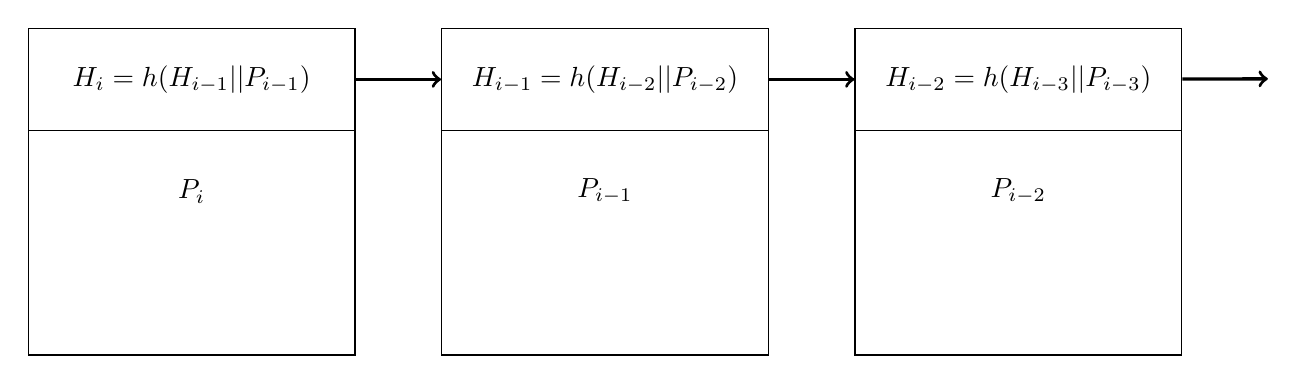
\begin{tikzpicture}


\coordinate(O1) at (0,0);
\node[below right=0cm of O1,draw, minimum width=4.15cm,minimum height=4.15cm,fill=white](block1) {$P_i$};
\node[below right=0cm of O1,draw, minimum width=4.15cm,minimum height=1.3cm,fill=white](hash1) {$H_i = h(H_{i-1} || P_{i-1})$};


\coordinate(O1) at (5.25,0);
\node[below right=0cm of O1,draw, minimum width=4.15cm,minimum height=4.15cm,fill=white](block2) {$P_{i-1}$};
\node[below right=0cm of O1,draw, minimum width=4.15cm,minimum height=1.3cm,fill=white](hash2) {$H_{i-1} = h(H_{i-2} || P_{i-2})$};

\coordinate(O1) at (10.5,0);
\node[below right=0cm of O1,draw, minimum width=4.15cm,minimum height=4.15cm,fill=white](block3) {$P_{i-2}$};
\node[below right=0cm of O1,draw, minimum width=4.15cm,minimum height=1.3cm,fill=white](hash3) {$H_{i-2} = h(H_{i-3} || P_{i-3})$};

\draw[->, very thick] (hash1) -- (hash2);
\draw[->, very thick] (hash2) -- (hash3);
\draw[->, very thick] (hash3) -- (15.75, -0.65);
\end{tikzpicture}
\caption[A simple blockchain]{A graphical representation of a Blockchain.
Each block consists of a payload $P_i$ and a hash $H_i$ of the previous block.
Here $h$ is the hash function and $||$ denotes concatenation.}
\label{Blockchain}
\end{figure}

\subsection{Bitcoin}

The idea for Bitcoin first appeared in 2008 with a paper by the (still unidentified) Satoshi Nakamoto\cite{bitcoin-whitepaper}.
It is based on a continuously growing blockchain, with transactions stored as payloads.
Creating a new block requires solving a computationally difficult problem.
The longest valid chain of blocks is considered to be the correct one and this allows a distributed consensus to be formed,
giving an order to transactions.

The first Bitcoin client was released in 2009, again by Satoshi Nakamoto.
Since then it has been maintained by the community and several other similar cryptocurrencies have emerged.


Each user in Bitcoin has a public/private key-pair, with the public key also acting as an address.
Coins may be sent to any address, but spending coins requires the signing of the transaction with the user's private key.

Bitcoins are created when new blocks are minted by `miners', who get a Bitcoin reward for every block they create.
These mining nodes form the backbone of the network and will check the validity of every transaction.

Every transactions consist of a list of input coins, along with proofs of ownership (normally just a digital signature)
and a list of output coins, along with a description of what is required to spend them in the future (again normally a digital signature from some address).
The transaction is then signed with the user's private key and broadcast to the network.
Each node in the network verifies that each of the input coins is valid (the unlocking proof is valid
and the coin has not already been spent), that the signature is valid for that address and that the total value of the inputs is at least that of the outputs.
The transaction will then be added to the next block, which each node verifies before beginning work on further blocks.


\subsection{Ethereum}


Ethereum is another cryptocurrency, initially proposed in late 2013\cite{eth-whitepaper}.
It is based on the same ideas as Bitcoin, but extended with a Turing complete language
embedded in the protocol.
There are also several other changes, primarily intended to improve performance, however they are not relevant here.
Its base currency is known as Ether.

An address controlled by a piece of code is referred to as a \textit{smart contract}.
The contract analogy holds in the sense that the contract cannot be modified or removed by
its owner or any other party, except in ways defined in the contract itself.
As such, if you put money (Ether) into a smart contract, you are bound to its terms.

The contract code is stored on the blockchain and whenever a transaction is sent to its address the code is executed,
and may in turn call other contracts or send Ether to other addresses.
In this way the code becomes part of the block verification process run by all nodes in the network.







\section{Smart contracts}

%\subsection{Contract structure}

A contract is defined by its bytecode and a JSON-style document describing its interface.
This interface defines the entry points into the contract and what arguments these entry points expect.
One of these functions may be a constructor, which is run when the contract is first deployed to the blockchain.

\subsection{Gas}

To compensate miners for running the code (and to prevent denial of service attacks) each step of execution in a contract costs money to the transaction's sender.
Any transaction intended for a contract should include some amount of `gas' which must be paid for in Ether.
The contract code is then executed until it either terminates or runs out of gas.
%There is a gas limit on transactions which is currently about four million gas, this limit is variable and is
%controlled by the miners.

To give some context, one gas is currently worth $1.8 \times 10^{-8}$ Ether and one Ether is currently worth \textsterling34.93\footnote{
All currency values are given in Pounds Sterling, correct on 2017-04-11.}.
This means that submitting a transaction with the maximum amount of gas (4000000) would cost about \textsterling2.48.

\subsection{The EVM}


I'll refer to the language used by Ethereum as EVM (Ethereum Virtual Machine) bytecode.
It is a stack based bytecode with a word size of 256 bits (the output size of the hash function used by Ethereum and the size of an address).

%When executing contracts have access to three types of memory with varying costs, permanent storage in particular is very expensive:
Contracts have access to both temporary memory and permanent storage, which allows state to persist between calls to the contract.
Temporary memory is cheap to access (2-3 gas), whilst permanent storage is much more expensive (20000 gas per allocation).
Sending data to contracts is similarly expensive; sending a 1kb file to a contract costs about 2.25 million gas or about \textsterling1.40.
Further details on gas costs can be found in Appendix \ref{evm-mem}.

All data sent to or held by a contract is public knowledge as it is shared between all nodes.
As such private data must be stored off-chain or encrypted before sending.
The hashes of the last 256 blockchain blocks are available to contracts in the EVM, not including that of the current block.

\subsection{Relevant limitations of Ethereum}

\begin{itemize}
\item No external source of randomness can be used as the computation must be deterministic,
however block hashes may be used for this purpose as they cannot be easily predetermined.
I will use block hashes as a source of randomness to generate a key.

\item All data sent to or held by a contract is public knowledge as it is shared between all nodes.

\item Extensive computations are expensive.

\item Sending data to contracts is expensive, as is storing it once it arrives.
\end{itemize}


\subsection{Solidity}

Solidity is a high-level language designed for contract creation that compiles to EVM bytecode.
Originally proposed in 2014, Solidity is a statically typed object oriented language with JavaScript-like syntax\cite{solidity-proposal}.
The language is still in development and there are some limitations not present in EVM bytecode, like the lack of nested dynamic arrays and array slicing\cite{solidity-docs}.

As part of my preparation I learnt to use Solidity and have since used it to write the contract.
The full contract code is included in Appendix \ref{app-contract} if you wish to see an example of Solidity code.


\section{Public Proofs of Retrievability}

A Proof of Retrievability (PoR) is proof that one can access a file.
I've also seen these methods referred to as Provable Data Possession in the literature.
In this section I give a formal definition and go through the algorithm that I will
later use to implement the system.

Another PoR method will be discussed when I look at extensions.

\subsection{Definition}


For a contract implementation a Public Proof of Retrievability (PPoR) is required, in which the verifier does not have access to the file,
or any other private information.
I formalise this concept using a simplified version of that used by Juels and Kaliski\cite{ecc-por}.

A PPoR is described by a three-tuple of deterministic polynomial-time algorithms:


\begin{itemize}
\item $\texttt{extract}(F) \to {H}$

Takes a file, $F$, and produces a handle, ${H}$, for this file.


\item $\texttt{generate\_proof}(F, \kappa) \to r$

From a file $F$ and key $\kappa$ generate a Proof of Retrievability $r$.

\item $\texttt{verify}({H}, \kappa, r) \to \{0, 1\}$

Verify the proof $r$ using $\kappa$ and ${H}$, but without access to the original file $F$.
It must be the case that $\texttt{verify}(\texttt{extract}(F), \kappa, \texttt{generate\_proof}(F, \kappa)) = 1$
\end{itemize}



\subsection{Security game}\label{security-game}

A security game for this definition consists of a verifier and a polynomial time attacker.
Intuitively the attacker is trying to demonstrate that they hold the file whilst not actually doing so.

The attacker is initially given the file $F$, may process it, then must discard down to store at most $g(|F|)$ bits of data (where $|F|$ is the size of the file).
The verifier and attacker are then both given ${H} = \texttt{extract}(F)$ and the same random key $\kappa$.
The attacker wins if they can output an $r$ such that $\texttt{verify}({H}, \kappa, r) = 1$.
We say a PPoR is secure under $g$ if $\Pr (\texttt{verify}({H}, \kappa, r) = 1)$ is negligible for sufficiently large files $F$.

If the attacker can store the whole file ($g(n) \geq n$) then the attacker can win every time by storing the whole file $F$ and choosing $r = \texttt{generate\_proof}(F, \kappa)$.
A perfect PPoR scheme would be secure for any $g$ which grows more slowly than the identity function (all $g \in o(\lambda n. n)$).
We wish to minimise the chance the attacker will succeed when they cannot store the whole file.

Note that the key $\kappa$ must be generated after the attacker discards down to $g(|F|)$ bits.
This prevents the attacker from computing $r$ using $F$ and just storing the proof if $|r| < g(|F|)$.


\subsection{Expected profit}

For this project I also look at the expected profit of an attacker per unit of storage used,
rather than just security under any particular quantity of storage given by $g$.

As originally proposed the system I construct pays out a fixed value $X$ on the submission of a correct proof.
A more practical implementation (and one I have completed as an extension) requires that the storing node pays a deposit
as a promise that they will keep the file. This means that failing to provide a proof incurs a loss of some $L$ Ether,
which can make PPoR schemes practical to use even if they do not provide perfect security under the above definition.


\subsection{Compactness}

In a contract implementation the file handle, ${H}$, and the proof, $r$, must both be sent to the blockchain.
Therefore for a scheme to be practical both ${H}$ and $r$ must be small in size.
Since the \texttt{verify} algorithm must run in a contract, it should also be as fast as possible.


A very simple PPoR scheme is to require the whole file as proof:
\begin{itemize}
\item $\texttt{extract}(F) = F$

\item $\texttt{generate\_proof}(F, \kappa) = F$

\item $\texttt{verify}({H}, \kappa, r) = ({H} == F)$
\end{itemize}
This is secure under, for example, $g(n) = \log(n)$, but ${H}$ and $r$ are both linear in $|F|$
so this cannot be used in practice.

One might imagine we could use a keyed hash function ($h_k$) to generate the proof
i.e. $\texttt{generate\_proof}(F, \kappa) = h_\kappa(F)$.
This has only shrunk the size of the proof $r$ however, as we still need ${H}  = F$ in order to perform the verification.


\subsection{Chunks}\label{por-chunks}

All Proofs of Retrievability I discuss going forwards act on files split up into fixed-size chunks\footnote{
In my proposal I referred to file chunks as file blocks, however this was too easily confused with blockchain blocks.}.
I use the following notation:
the file $F$ of size $|F|$ is split into $m$ chunks, $\{F_1, \ldots, F_m\}$, each of size $C$.

One way to implement a PPoR is to split the file into chunks and hash each of these chunks.
This list of hashes is the file handle ${H}$.
The key $\kappa$ is used to select a chunk and the proof is then that chunk.
The proof can be verified by computing the hash of that chunk and comparing it to the entry in ${H}$.

\begin{itemize}
\item $\texttt{extract}(\{F_1, \ldots, F_m\}) = \{h(F_1), \ldots, h(F_m)\}$


\item $\texttt{generate\_proof}(\{F_1, \ldots, F_m\}, \kappa) = F_{\kappa \mod m}$

\item $\texttt{verify}({H}, \kappa, r) = h(r) == {H}[\kappa \mod m]$
\end{itemize}

For this algorithm the size of ${H}$ is in $O(m)$ and the size of $r$ is in $O(C)$.
For fixed size chunks this means that $r$ is linear in $|F|$.
If the chunk size is allowed to vary with $|F|$ then, since $|F| = m \cdot C$, we can have ${H}$ and $r$ both linear in $\sqrt{|F|}$,
however it is possible to improve on this using Merkle trees.



\subsection{Merkle trees}

A Merkle tree is a tree-like data structure based on a hash function $h$ in which parent nodes are the hash of their concatenated children.
In our case leaf nodes will be the hash of a chunk of a file.

For example, if we have a file with four chunks $\left[F_1, F_2, F_3, F_4\right]$, we can build a Merkle tree by first hashing each chunk to obtain $\left[h(F_1), h(F_2), h(F_3), h(F_4)\right]$,
then combining adjacent nodes and finally computing the \textit{root hash}. 
This construction is most clearly represented in a graphical form as seen in Figure \ref{Merkle example}.


\begin{figure}[h]
\centering
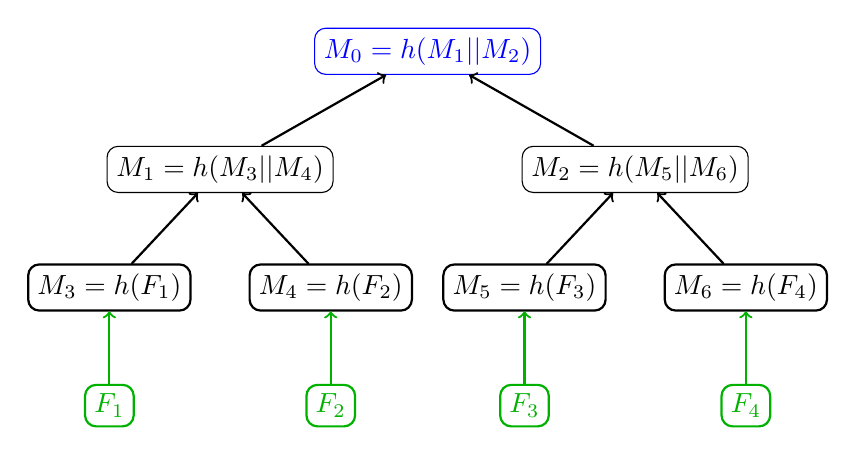
\begin{tikzpicture}[
	sibling distance=15em,
	every node/.style = {shape=rectangle, rounded corners,
	draw, align=center,
	top color=white, bottom color=white},
	level 2/.style={sibling distance=8em},
	level 3/.style={color=black!30!green},
	edge from parent/.style={<-,draw,thick}
]
\node[color=blue]{$M_0 = h(M_1 || M_2)$}
	child { node {$M_1 = h(M_3 || M_4)$}
		child { node {$M_3 = h(F_1)$}
			child { node {$F_1$} } }
		child { node {$M_4 = h(F_2)$}
			child { node {$F_2$} } }
	}
	child { node {$M_2 = h(M_5 || M_6)$}
		child { node {$M_5 = h(F_3)$}
			child { node {$F_3$} } }
		child { node {$M_6 = h(F_4)$}
			child { node {$F_4$} } }
	};
\end{tikzpicture}
\caption[A Merkle Tree]{A Merkle tree built from a file $F$ split into 4 chunks $[F_1, F_2, F_3, F_4]$..}
\label{Merkle example}
\end{figure}

The file chunks are not considered to be part of the Merkle tree when calculating depth, as such the tree in Figure~\ref{Merkle example} has depth 2.



\subsection{Merkle tree Public Proofs of Retrievability}\label{merkle-ppor}

Merkle trees provide a way to prove membership of a single chunk of a file in $O(\log(n))$ time and space,
whilst requiring the verifier to have only $O(1)$ information (the root hash).

A proof consists of a chunk of the file, and the chain of hashes needed reconstruct the path to the root hash,
as demonstrated in Figure \ref{Merkle proof}.

It is not computationally feasible to fake the proof just from the root hash; the file chunk and the relevant hashes (or the file to reconstruct them) are required.

To produce a proof of membership of chunk $F_3$, for example, we include $F_3$ in full.
We do not need to include $M_5 = h(F_3)$, since this can be calculated from $F_3$.
The aim of the proof is to demonstrate that the root hash can be derived from the file chunk, so we include $M_6$ and $M_1$.

A verifier then computes the hash of $M_5 = h(F_3)$, followed by $M_2 = h(M_5 || M_6)$
and finally $M_0 = h(M_1 || M_2)$. The verifier then compares $M_0$ to the known root hash and returns success if they are the same.

\begin{figure}[h]
\centering
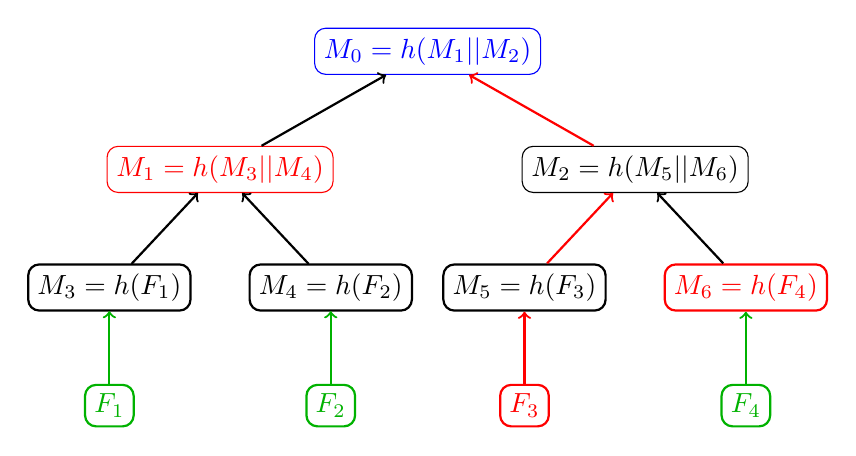
\begin{tikzpicture}[
	sibling distance=15em,
	every node/.style = {shape=rectangle, rounded corners,
	draw, align=center,
	top color=white, bottom color=white},
	level 2/.style={sibling distance=8em},
	level 3/.style={color=black!30!green},
	edge from parent/.style={<-,draw,thick}
]
\node[color=blue]{$M_0 = h(M_1 || M_2)$}
	child { node[color=red] {$M_1 = h(M_3 || M_4)$}
		child { node {$M_3 = h(F_1)$}
			child { node {$F_1$} } }
		child { node {$M_4 = h(F_2)$}
			child { node {$F_2$} } }
	}
	child { node {$M_2 = h(M_5 || M_6)$}  edge from parent[red]
		child { node[color=black] {$M_5 = h(F_3)$} edge from parent[red]
			child { node[color=red] {$F_3$} edge from parent[red]} }
		child { node[color=red] {$M_6 = h(F_4)$} edge from parent[black]
			child { node {$F_4$} } }
	};
\end{tikzpicture}

\caption[A Merkle Tree proof of membership]{A Merkle tree proof of membership for
a file $F$ split into 4 chunks $[F_1, F_2, F_3, F_4]$.
The parts of the tree which constitute the proof are coloured red.}

\label{Merkle proof}
\end{figure}


We can use this proof of membership to create a PPoR by making the chunk that the proof is for dependent on $\kappa$.
\begin{itemize}
\item $\texttt{extract}(F) = \texttt{root\_hash}(\texttt{Merkle}(F))$

\item $\texttt{generate\_proof}(F, \kappa) =
F_{\kappa \mod m} \,||\, [\text{Merkle tree hashes forming proof}]$

\item $\texttt{verify}({H}, \kappa, r) =
\texttt{extract\_root\_hash}(r) == {H}$
\end{itemize}



This scheme gives a constant size to ${H}$ and the size of the proof is $|r| = C + |h| \log_2(m)$ where $|h|$ is the size of one hash.
At first glance this may seem no better than hashing individual chunks, however if we fix the chunk size $C$ to a constant value then we can rewrite
the size of the proof in terms of $C$ and $|F|$ \[\displaystyle |r| = C + |h| \log_2\left(\frac{|F|}{C}\right) \in O(\log(|F|))\]
which gives logarithmic scaling with the size of the file.

%a logarithmic size to the proof ($|r| \in O(\log(m) + C)$).

This scheme certainly is not a perfect PPoR, an adversary storing only half the file and one hash value, for example, has a 50\% chance of being able to generate a valid proof.
However to successfully generate a proof the relevant chunk $(i \equiv \kappa \mod m)$ must be stored.
This means that the chance that an attacker can generate a proof is at most equal to the fraction of the file stored.
This is important because it means that it is never less profitable to store the entire file rather than some subset of it, in terms of expected profit per unit storage.






\section{Prior work}


\subsection{Filecoin}

Filecoin is a proposal for a Bitcoin-like cryptocurrency and distributed file system in one
that has a Proof of Retrievability component along with its proof of work function for block mining.
Its White Paper\cite{filecoin} points to work on compact Public Proofs of Retrievability by Shacham and Waters\cite{compact-por},
however as far as I could find Filecoin has never been implemented.

\subsection{Swarm}


Swarm is a proposed overlay system for a distributed file system (e.g. IPFS\cite{ipfs}), based on Ethereum.
At the time of writing Swarm is currently in alpha on the Ethereum public test chain\cite{swarm-alpha}.

Swarm has two parts, payment channels to incentivise file exchange and a system similar to the one designed here for incentivising long term storage,
which I will briefly discuss.

Swarm is built around fixed size chunks rather than files, so an owner would have to pay for each chunk of their file to be stored individually.
The proof system is similar to the one described in section \ref{por-chunks}, the file handle ${H}$ is just the hash of the chunk and the proof is the chunk itself.

To mitigate the gas cost of uploading chunks Swarm plans to use a receipt based challenge system.
File owners buy receipts as promises of storage and if they suspect that a node has failed to store their chunk then they issue
a challenge using the receipt and enough Ether to cover the chunk upload.
If the storing node fails to respond to this challenge then they lose their security deposit.
If no challenge is made then a proof is not required. This is explained further in Appendix \ref{app-challenge}.

Swarm's incentive scheme is also intended to be a backup way of recovering files if the normal file exchange system fails,
resulting in some deficiencies when viewed purely as an incentive system as I have done.
In particular their proof system is less efficient in terms of proof and file handle size and also requires interaction from the file owner.


%
%The approach I will take as some benefits over the one given here under the assumptions I operate under.
%%Should consider under challenge is always made for one chunk
%\begin{itemize}
%\item No interaction is required. The owner does not have to make the challenge themselves. Moreover an incorrect challenge will cost the owner in the Swarm scheme.
%\item Merkle tree proofs of retrievability are likely to be shorter, and require less information be held by the client, at least for large files.
%
%Consider the implementation used by Swarm, with a chunk size $C$ (4096 bytes in Swarm), and say the owner wants to ensure an entire file $F$ of size $|F|$.
%There will be $\frac{|F|}{C}$ chunks and the owner must therefore store $\frac{|F|}{C}$ receipts.
%The chunk hash and signature will both be 32 bytes in size (the hashing functions and Elliptic curve cryptography verification function available to the EVM uses 256 bit keys).
%The owner must store at least $64 \cdot \frac{|F|}{C}$ bytes. The proof for any given chunk is $C$ bytes, we assume the owner requests a proof for one random chunk.
%
%In comparison, in a Merkle tree scheme the owner stores nothing and the proof size is $C + 32 \cdot \log_2(\frac{|F|}{C})$.
%This encourages a chunk size of around 64 bytes. For a 1MB file the proof size is then 512 bytes.
%Choosing to make the proof size equal in the Swarm scheme (so $C = 512$ bytes) we find the owner must store $64 \cdot \frac{1 \text{MB}}{512 \text{bytes}} = 131072$ bytes,
%or about 13\% of the original file size. This can be reduced by increasing the chunk size, in exchange for higher transaction fees when a challenge is made.
%\end{itemize}
%
%The scheme used by Swarm does have a potentially significant advantage that transaction costs are very low if a challenge is never made.
%This makes sense for Swarm as we expect the owner to try and recover the files from the Swarm network before resorting to a challenge as insurance.
%As such the higher transaction fees are not a significant issue, though if this litigation procedure becomes common Swarm could benefit from building a 64 byte based Merkle tree
%from each chunk when considering receipts and litigation as this would decrease the proof size to 256 bytes.
%
%The scheme used by Swarm is simpler, just a single hash operation.
%While this is a good thing, to the EVM the extra complexity is cheaper than the larger transaction size.


%\section{Requirements analysis}

% Java, Eclipse, geth, Remix, test-chain



%\section{Planning}

\section{Requirements analysis}

I will implement the system as described in the introduction sections \ref{intro-scope} and \ref{intro-plan} using the Merkle tree Proof of Retrievability scheme
discussed above. This involves two components:
\begin{itemize}
\item The contract, which will be able to verify Merkle tree Proofs of Retrievability.
\item The proof generator, which must be able to extract the Merkle tree root hash and generate a valid Proof of Retrievability for a given file.
\end{itemize}

The contract should make it easy to change file specific variables so that a version could be deployed for any file.
Similarly is should be easy to change the target file, chunk size and key for proof generation.

%I also have several extensions I would like to complete given time.

\section{Tools and libraries}

I will implement the proof generator in Java using the Eclipse IDE.
I plan to use the following libraries:
\begin{itemize}
\item Apache Commons CLI for creating a command line interface (Apache license)
\item JUnit for unit tests (Eclipse Public License)
\end{itemize}
In addition I introduced the library RNRT SAPHIR (MIT-like and BSD-like licenses) during the implementation phase
for reasons I will discuss in section \ref{impl-keccak}.

For developing the contract I will use the language Solidity using the online IDE Remix\cite{browser-solidity}.
I will test it on a private chain\footnote{That is, a private Ethereum blockchain with all blocks and transactions generated locally.}
using the go-ethereum client \texttt{geth} and the solidity compiler \texttt{solc}.


\section{Planning}\label{plan}

I have planned out the behaviour of each component.
In particular I wanted to detail the interface between the proof generator and the contract
to ensure they will work together once complete.

The following is a summary of the plan I made towards the end of the preparation stage to allow me to begin implementing the system.
It also acts as a reference for the variables I will use throughout the report, though I will continue to define any that have not appeared before now.

\begin{itemize}
\item $F$ is the file the contract is for.
\item $m$ is the number of chunks in $F = [F_1, F_2, \ldots, F_m]$.
\item $C$ is the size of those chunks.
\item $M$ is the smallest power of two greater than or equal to $m$.
\item $H$ is the handle of the file, in this case root hash of the Merkle tree of the file $F$ zero-padded to $M$ chunks in size.
\item $T_0$ is the block the contract is created on.
\item $t$ is the number of blocks the contract waits before becoming active.
\item $X$ is the amount of ether the contract holds initially.
\item $\kappa$ is the block hash of block $T_0 + t$, which acts as the key for the PoR.
\item $i$ is the chunk of the file a proof for is required, I take $i \equiv \kappa \mod m$.
\end{itemize}

The contract should reject a proof submission if:

\begin{itemize}
\item The contract has already paid out its reward.
\item The current block number is $\leq T_0 + t$.
\item The current block number is $> T_0 + t + 256$.
\item The proof is invalid.
\end{itemize}

The proof itself, $r$, is a sequence of bytes containing the selected file chunk $F_i$ and the other hashes from the Merkle tree required to recover the root hash.


\section{Review of the preparation stage}

I achieved all of my goals for the Preparation stage of the project.
I am happy with the planning I did, the contract and the proof generation components worked together successfully with only very minor changes.




	%%%%%%%%%%%%%%%
	%%%  IMPLEMENTATION %%%
	%%%%%%%%%%%%%%%

\chapter{Implementation}

\section{Project structure}
\label{pseudo-code}

There are three algorithms that need to be implemented:
\begin{itemize}
\item Extract -- Find the Merkle tree root hash (${H}$) from $F$. This is uploaded to the blockchain as part of the contract.
\item Generate proof -- Given a file $F$ and a key $\kappa$ create a Proof of Retrievability.
\item Verify proof -- Given a root hash ${H}$, a proof $r$ and key $\kappa$ determine whether the proof is valid.
\end{itemize}

I will code the first two in Java.
The algorithms for finding a Merkle tree root hash and for a proof of membership are similar
and in my implementation a lot of the code is reused, so I've treated these as one component for implementation purposes.

The verification is part of the contract, written in Solidity.

\begin{figure}[H]
\centering
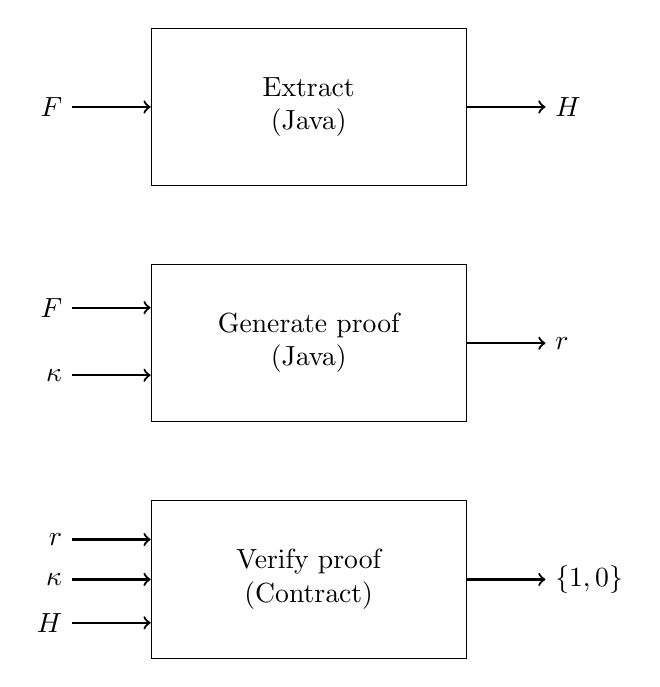
\begin{tikzpicture}
\coordinate(O1) at (0,0);

\node[below=0cm of O1, draw, minimum width=4cm, minimum height=2cm, align=center](a) {Extract\\(Java)};
\node[left=1cm of a](aF) {$F$};
\node[right=1cm of a](anu) {${H}$};

\node[below=3cm of O1, draw, minimum width=4cm, minimum height=2cm, align=center](b) {Generate proof\\(Java)};
\node[above left=-0.8cm and 1cm of b](bF) {$F$};
\node[below left=-0.8cm and 1cm of b](bi) {$\kappa$};
\node[right=1cm of b](br) {$r$};
\node[right=1cm of bF](bFb) {};
\node[right=1cm of bi](bib) {};

\node[below=6cm of O1, draw, minimum width=4cm, minimum height=2cm, align=center](c) {Verify proof\\(Contract)};
\node[above left=-0.7cm and 1cm of c](cr) {$r$};
\node[left=1cm of c](ci) {$\kappa$};
\node[below left=-0.7cm and 1cm of c](cnu) {${H}$};
\node[right=1cm of c](cbool) {$\{1, 0\}$};
\node[right=1cm of cr](crc) {};
\node[right=1cm of cnu](cnuc) {};


\draw[->, thick] (aF) -- (a);
\draw[->, thick] (a) -- (anu);
\draw[->, thick] (bF) -- (bFb);
\draw[->, thick] (bi) -- (bib);
\draw[->, thick] (b) -- (br);
\draw[->, thick] (cr) -- (crc);
\draw[->, thick] (ci) -- (c);
\draw[->, thick] (cnu) -- (cnuc);
\draw[->, thick] (c) -- (cbool);
\end{tikzpicture}
\caption[Project structure]{The three functions that need to be implemented.}
\label{project-structure}
\end{figure}


\subsection{Extract}

To build the Merkle tree I split the file $F$ into $m$ chunks of size $C$, zero padding the final chunk if necessary.
I then append all-zero chunks to the file until the total number of chunks, $M$, is a power of two.
The Merkle tree is then built over this extended chunk set and will have depth $\log_2(M)$.
The chunk size $C$ is controlled by a variable and can be easily modified.

I feel that these three functions are sufficiently important to include in the report as pseudo-code.
Here the hash function is \texttt{h} and \texttt{readChunk()} that returns the next chunk in the file,
implicitly keeping track of its current position.

\lstset{
breaklines=true,
basicstyle=\ttfamily\small,
tabsize=4
}
\begin{lstlisting}
fun merkle(depth) 
    if (depth == 0) 
        return h(readChunk());
    else 
        return h(merkle(depth - 1) || merkle(depth - 1));
    

\end{lstlisting}

\subsection{Generate proof}\label{pseudo-proof}

The proof generation acts on the same $M$ chunk Merkle tree as the root hash algorithm.
The key $\kappa$ is the hash of block number $T_0 + t$ and the chunk selected to be included in the proof is $i \equiv \kappa \mod m$, note that
the padding chunks cannot be selected for proof.

The proof itself is a sequence of bytes containing the selected file chunk $F_i$ and the other hashes from the Merkle tree required to recover the root hash.

\vspace{1em}

\begin{figure}[H]
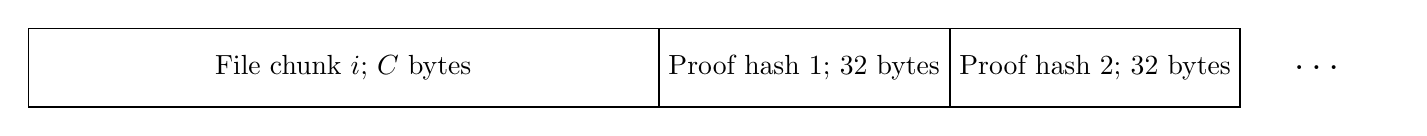
\begin{tikzpicture}

\node[draw,minimum width=8cm,minimum height=1cm](chunk) {File chunk $i$; $C$ bytes};
\node[right=0cm of chunk,draw,minimum width=3cm,minimum height=1cm](hash1) {Proof hash 1; 32 bytes};
\node[right=0cm of hash1,draw,minimum width=3cm,minimum height=1cm](hash2) {Proof hash 2; 32 bytes};
\node[right=0cm of hash2,minimum width=2cm,minimum height=1cm](hash2) {\Large\ldots};

\end{tikzpicture}
\caption[Proof structure]{A representation of the structure of my Merkle tree based PoR.}
\label{fig-proof}
\end{figure}

The proof generation algorithm for the \texttt{i}th chunk of the file can be expressed as a recursive function,
making use of the \texttt{merkle} root hash function defined above.

\begin{lstlisting}
fun proof(depth, i)
    if (depth == 0)
        readChunk();
    else
        M = 2^(depth - 1);
        if (i < M)
            return proof(depth - 1, i) || merkle(depth - 1);
        else
            tmp = merkle(depth - 1);
            return proof(depth - 1, i - M) || tmp;
\end{lstlisting}



\subsection{Verify proof}

To verify the proof, one first hashes the first $C$ bytes to calculate $h(F_i)$, the hash of the file chunk.
This hash is then concatenated with the next hash in the proof,
this new value is then hashed and this is repeated $\log_2(M)$ times (the depth of the Merkle tree).
A valid proof is one that results in the root hash as the final value.
The order in which the hashes are concatenated ($A \,||\, B$ or $B \, || \, A$) depends on $i$.
This can be visualised as a walk up the Merkle tree or
equivalently as depending on the binary representation of $i$, from least to most significant bit.

The algorithm can be expressed as follows, recalling the structure of the proof from Figure \ref{fig-proof}.
Here \texttt{array[$a$, $b$]} denotes array slicing, representing the sub-array of \texttt{array} between positions $a$ and $b$.

\begin{lstlisting}
fun validate(chunkSize, rootHash, proof, i)
    
    depth = (proof.length - chunkSize) / hashLength;
    hash = h(proof[0, chunkSize]);
    int positionInProof = chunkSize;
    
    for n in 0..(depth-1)
        otherHash = proof[positionInProof, positionInProof + hashLength];
        if (i % 2 == 0)
            hash = h(hash || otherHash);
        else
            hash = h(otherHash || hash);
        
        i /= 2;
        positionInProof += hashLength;
    
    return hash == rootHash;
\end{lstlisting}

The full Java code for these three functions can be found in Appendix~\ref{app-java}.


\section{Alterations from proposal}
\label{impl-changes}

I made two minor changes to the original design as the project progressed.

\subsection{SHA256 $\to$ SHA3 KECCAK}\label{impl-keccak}

I mentioned using the SHA256 hash function in the proposal, however I am now using a different hash function, KECCAK-256.
This is due to me misunderstanding the Solidity documentation when I read it at the time.
Whilst SHA256 is available in EVM bytecode it is in the form of a precompiled contract
so as not to use up the limited number of possible EVM opcodes.

As I'll mention later array slicing is not yet implemented in Solidity, so at points I used in-line assembly to improve efficiency.
In this assembly language SHA256 is not as easily available, so instead I switched to SHA3's KECCAK-256 function, which is available as a true opcode in the EVM\footnote{
The KECCAK-256 function is confusingly referred to as \texttt{sha3} in EVM bytecode. Whilst KECCAK-256 is part of SHA3 they are different functions.}.
The output is the same size so it is a drop in replacement in the contract, the only downside is having to bring in an external library
to handle it in Java (RNRT SAPHIR), whilst SHA256 was available from the standard library.

\subsection{Block hash}

This is an implementation detail. The proposal mentioned the use of the block hash of block number $T_0 + t$ as the key value for proof generation and verification.
The block hash of the current block is not available\footnote{
The `current block', in which the code is executing, does not actually exist
when the code is first run during the block's construction.}, so the contract actually used the block hash of block $T_0 + t - 1$ instead.



\section{Security considerations}

There are several edge cases and other implementation details I had to consider to ensure the contract behaves as expected.
The correctness of the proof algorithm has already been considered and
I will assume that the Ethereum network and the hashing algorithm are not compromised.

\subsection{Block hash as random number} \label{sec-block-hash}

I use the block hash of some block that has not yet been created when the contract is deployed as the key $\kappa$.
If someone could control the block hash then they would control the key and would have an advantage if they were to try and cheat my system.
Anyone wishing to control the block hash would have to generate blocks ahead of the main network
and discard them until they found one they wanted.
Discarding blocks means that the block reward is lost,
however in Ethereum an `Uncle block' (see Appendix \ref{app-uncle}) can still be produced and a reduced reward can be claimed, $\frac{7}{8}$ 
of the normal 5 Ether.

This means a node is sacrificing at least 0.625 Ether (about \textsterling21 at current prices)
to re-roll a new random block hash.
The node will therefore never discard a block if the reward is less than this loss, that is $X < 0.625$ Ether.\footnote{Assuming they have less than 50\%
of the total mining power, at which point they would control the network anyway.}

If this were to become a problem, then one solution would be to allow the file owner to pick the chunk (or set of chunks)
that a proof is required for.


\subsection{File length is not a multiple of chunk size}
\label{file-len-chunk-size}

In this case there is less information contained in the final chunk of the file, as it is zero padded in my implementation.
This means storing the last chunk of the file is slightly more profitable (per byte stored), as it uses less space.

One way to solve this would be to pad files with random bits to a multiple of the chunk size before using the contract,
however this would mean the file's original length would be needed to recover the file, so I have not done this in my implementation.
Another solution would be to reduce the chance that the last chunk will be selected for a proof in accordance with its relative size.
%This problem is partially solved by requiring a storing node to pay a deposit as a promise they will keep the file.
%** Could reduce probability of being selecteds

\subsection{Number of chunks, $m$, is not a power of two}
\label{file-len-chunk-num}

The number of leaf nodes in the Merkle tree (in my implementation) must always be a power of two.
The extra chunks are treated as all zero when building the tree, though they will never be selected for proofs.
%This was done for simplicity of implementation.

This means that if you are only storing a subset of the chunks, plus extra hashes to allow proof construction,
then some will require slightly less extra data.
However it is still more profitable per chunk stored to keep the whole file and be able to reconstruct the Merkle tree as required.

%If the actor stores the whole file then the payout per chunk is $\frac{X}{m}$.
%If the actor were to only store $n < m$ chunks then they must store a strictly positive amount of extra data, $\epsilon$, to be able to reliably construct a valid proof for those $n$ chunks.
%The chance that one of these $n$ chunks is chosen is $\frac{n}{m}$.
%Therefore the expected payout per chunk is $\frac{n}{m} \cdot \frac{X}{n + \epsilon} = \frac{X}{m + \epsilon'} < \frac{X}{m}$
%and the actor will always store the whole file.
%
%This breaks down if the actor cannot store the whole file in which case it can cause some sets of chunks to be more valuble than others.

%This edge case is a good reason to implement the lock-in extension (section \ref{ext-lockin}).

\subsection{Block hash availability}

The last 256 block hashes are available to code executing in the EVM, not including that of the current block.
The EVM opcode that retrieves a block hash fails silently if that block is not available, returning 0.
As such the block hash used as the key $\kappa$ must exist before the contract becomes active,
and the contract must deactivate 256 blocks later, rejecting further proof submissions.

There are methods to get round this limit, however with a block time averaging 14 seconds
256 blocks is about one hour, which is plenty of time to create a proof and submit the transaction.

\subsection{Multiple rewards}

If the content of the file is very important to the owner then they may want multiple nodes in the network to keep copies of the data.
Simply allowing the contract to pay out to multiple Ethereum addresses will not work as one node could store the file once and claim all the rewards
using different addresses.
A better way for the owner to increase their confidence in the files security would be two encrypt the file with different keys and
upload multiple versions of the file with separate contracts.



\section{Software engineering practices}

\subsection{Tools}

For Solidity I used the online IDE (Integrated Development Environment) Remix\cite{browser-solidity}, as suggested by the documentation, for developing the contract.
The IDE has the ability to compile and deploy the contract to an emulated private chain for development.
It also includes a debugger, which I made extensive use of, in part to make up for the lack of traditional print statements.

For Java I used the Eclipse IDE, which I am familiar with, along with its integrated debugger.

\subsection{Design}

During the design phase I put emphasis on fully defining the interface between the contract and the Java part of the project, which allowed me to develop them separately.
This proved very useful and they worked together with no problems after the hash function change.

When developing the contract I made sure I was aware of best practices regarding security from the documentation\cite{solidity-docs-security}
and I believe my code adheres to them.


\subsection{Testing}

I wrote unit tests for the Java code as I was developing it, using the JUnit framework.
The tests were helpful in finding bugs as I continued to implement this part of the project.

I felt that traditional unit tests were not appropriate for the contract as its only complicated functionality (proof verification)
depended on the Java code to run and there was no way to integrate tests with the online IDE.
Instead I extended the Java program to fill in constant values in a skeleton version of the contract and wrote a deployment script
for the go-ethereum command line client, \texttt{geth}, that allowed me to easily test the contract with different files
by inserting assertions into this script.

\section{Java proof generator}

% The following main components

%Detailed class structure, cli, what libraries

This part of the project was fairly straightforward due to my detailed plan and familiarity with Java.
I wrote the code to extract the Merkle tree root hash and generate proofs first and wrote the contract generator later when I was starting to test the contract.

\subsection{Class structure}
\subsubsection{ChunkStream}

This class is a wrapper around a Java file stream that abstracts it into a stream of fixed size chunks.
This component can the be easily tested and it keeps IO code out of the rest of the codebase.
I wrote several unit tests for the ChunkStream class, particularly checking behaviour in edge cases like the last chunk of a file,
files that have a number of chunks that is not a power of two and files smaller than one chunk.
It extends an abstract class which has other implementations, for example random or all-zero files, which I used when testing other components.

\subsubsection{Merkle}
This class is the core of the base project, it wraps around a ChunkStream and has methods for finding the root hash of a file and generating proofs.

I first implemented this class by building the whole Merkle tree in memory upon initialisation,
however this can use large amounts of memory since the size of the tree grows linearly with the size of the file.
Instead I have rewritten this part of the code so that the root hash and proof construction is done using a recursive function using only $O(\log(|F|))$ space,
which is the one expressed as pseudo code in section \ref{pseudo-proof}. Some of that Java code from this class can be found in Appendix~\ref{app-java}.

In terms of testing I implemented the verification procedure in Java
and used it in several unit tests to ensure the proof is correct, since that is the interface with the contract.


\subsubsection{ContractGenerator}

Whilst I was developing the contract I found that the process for deploying the contract to a local blockchain was very cumbersome, so
I added additional code to the Java part of the project to generate contracts by filling in file specific constants like the number of chunks and the Merkle tree root hash.
The contract is then packed into a JavaScript file for the \texttt{geth} Ethereum client to run, which deploys the contract ready for testing.
This made it much quicker to test the behaviour of the contract on different files as well as making it possible to write integration tests by altering the deployment script.

\subsection{Command line interface}

I added a simple command line interface to the program as I built it allowing me to easily test the code.
Using the interface I can choose between generating a contract, deployment script or proof, and various settings
like file name and block hash.
I later added the extensions to this interface as optional flags.

I used the Apache Commons CLI library for this.


\section{Contract}

I wrote the contract in Solidity.
Although there is less code than in the Java part of the project, the contract took longer to write due to my unfamiliarity with the language and
some issues which I had to resolve as the project progressed.


\subsection{Structure}

For ease of writing and reading the contract is split into two main functions, though they are just called sequentially when
the main entry point \texttt{submitProof} is run.
There are also a few small functions that provide information about the contract's state for testing, as well as a simple
constructor (which is run when the contract is deployed) which records the initial block number $T_0$ and address of the contract's owner.

\subsubsection{validToCall}

This function performs the checks listed in the design plan of section \ref{plan}.
\begin{itemize}
\item The block number is $> T_0 + t$.
\item The block number is $\leq T_0 + t + 256$.
\end{itemize}

\subsubsection{validateProof}

This function validates the Merkle tree Proof of Retrievability against the stored root hash using the \texttt{validate} algorithm in section \ref{pseudo-code}.
The proof is received as a fixed-size array, so the contract must be altered for different files.
Fixed size arrays are more performant, easier to use in the in-line assembly and preclude any potential bugs from submitting different size proofs than
expected.



\section{Difficulties with the contract implementation}

I encountered several problems during implementation of the base contract, however I was able to overcome them with no major issues.
I detail a few of these problems here.

Ethereum itself is in `beta', expecting breaking changes\footnote{
By `breaking changes' I mean that the network is planning to undergo what are known as `hard forks', changing the block validation procedure.
This means that, at the point of the hard fork, future blocks will not be considered valid under the current block validation algorithm and therefore all miners
must update to the new version or they will be left behind on a different chain.},
and its ecosystem is young and still developing.
I knew this before proposing the project and planned in extra time to deal with problems implementing and testing the contract.

\subsection{Documentation}

Though there is central documentation for Solidity which has been very helpful, it is brief and incomplete in places and this slowed down my development of the contract.
For example there is little detail on lesser used keywords (like \texttt{internal}, \texttt{constant} and \texttt{modifier}), especially when compared to the usually very thorough documentation for the Java standard library.

\subsection{Array slicing}

The contract receives proofs as arrays and has to hash slices (subsections) of those arrays.

Solidity does not support array slicing (that is, taking part of an array by using a pointer to the same memory rather than making a copy).
I wanted to avoid making a copy for performance reasons.
For this reason the contract uses some in-line assembly code to manipulate array pointers.


%Anecdotally, this is also the case in Java, though it can be worked around with wrapper objects like \texttt{ByteBuffer}.

%\subsection{Libraries}
%
%% not reall improtant?
%Solidity does not come with a standard library. The only extra functions available are those implemented as EVM opcodes or precompiled contracts.
%There is no central place for Solidity libraries (* * * was created while my projects was in development).

%SHA3/KECCAK confusion.

\subsection{Tooling}

There is an online IDE for Solidity\cite{browser-solidity} which is suggested by the documentation.
This generally worked well, however code execution is very slow and would sometimes hang or run out of memory.
Being JavaScript based it cannot deal with the EVM's 256-bit word size natively, so large arguments have to be input as zero-padded hex strings.

As far as I can tell the files generated by the offline compiler \texttt{solc} cannot be interpreted by \texttt{geth}, the Ethereum command line client.
A workaround is to call the Solidity compiler from within \texttt{geth}'s JavaScript console,
however JavaScript does not support multi-line strings.
For this reason my Java contract generator removes newlines from contracts and creates a script to deploy them from \texttt{geth}.
This worked in most of the time because Solidity does not assign any particular meaning to newlines, except in the case of line comments (\texttt{//}) and in-line assembly,
which does not use semicolons to separate expressions.



%%later
%\subsection{Limitations of the EVM}
%
%% No ECC primitives
%
%% No modexp precompile
%
%\subsection{Java and Solidity}
%
%There were a few hard to find bugs in the project that resulted from interoperating between Java and Solidity.
%
%Java's \texttt{BigInteger}, which I make extensive use of in the RSA extension gives a two's complement representation
%when asked for a \texttt{byte[]} representation, which was not useful to me as I was dealing with modular arithmetic and did not need negative numbers.
%This means in particular that, for example, a 256 bit number may take 33 bytes to represent, and attempting to store it in a 32 byte array
%will not produce the desired result in some cases.
%It also becomes an issue when trying to hash \texttt{BigInteger}s in a way that is consistent with Solidity.
%Java \texttt{BigInteger}s have to be converted to byte arrays and then padded or shortened before hashing and reconstructing a \texttt{BigInteger}
%using the hash result as magnitude to produce the desired result.
%To convert to a format that is understood by the JavaScript interface it is necessary to convert it to hex and left pad the result with zeroes
%(and put it in a string starting with \texttt{0x}), because values are otherwise implicitly right-padded to 32 bytes by default.


\section{Configuration}

\subsection{Chunk size}

\subsubsection{Performance of proof generation}

In general larger chunk sizes improve performance simply because the Merkle tree will have fewer nodes and so take less time to build.

\subsubsection{Proof size} \label{chunk-size-proof-size}

Recall that the proof is the chunk concatenated with all the hashes required for a Merkle tree proof of membership.

Let the chunk size be $C$ bytes.
The number of chunks for a file $F$ is therefore $\frac{|F|}{C}$.
The depth of the Merkle tree is $\left\lceil\log_2\left(\frac{|F|}{C}\right)\right\rceil$.

We use a hash algorithm with 256-bit (32 byte) output, so the proof size is
\[|r| = C + 32 \cdot \left\lceil\log_2\left(\frac{|F|}{C}\right)\right\rceil\]

\begin{figure}[h]
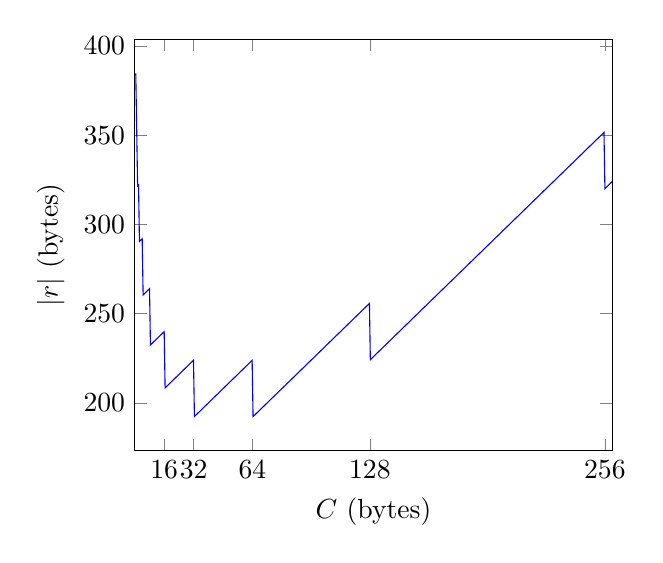
\begin{tikzpicture}
  \begin{axis}[ 
    xmin=0, xmax=260,
    xlabel={$C$ (bytes)},
    ylabel={$|r|$ (bytes)},
    domain=0:260,
    samples=522,
    xtick={16, 32, 64, 128, 256},
    scale only axis,
    width=0.5\textwidth,
  ]
    \addplot[color=blue,mark={}]{x + 32 * ceil(log2(1024 / x))}; 
  \end{axis}
\end{tikzpicture}
\caption[Chunk size graph]{Proof size against chunk size for a 1kb file.}
\label{impl-graph-chunk-size}
\end{figure}


The size of the proof will always be smallest when $\frac{F}{C}$ is a power of two due to ceil operation.
If we require $|F|$ to be a power of two then it follows that $C$ is also a power of two when $|r|$ is minimised.
Restricting $C$ to be a power of two means that we can eliminate the ceil operation and hence
\[|r| = C + 32\log_2(|F|) - 32\log_2(C)\]
so we can simply minimize $C + 32\log(C)$ with respect to $C$, finding that 32 and 64 bytes both give minima as shown in Figure \ref{impl-graph-chunk-size}.
Since proof generation benefits from larger chunk sizes I have chosen 64 bytes as the default chunk size.

A more complete analysis is included in Appendix~\ref{app-chunk-size}.

\section{Extensions}


I have completed the following extensions, including the necessary modifications to both the contract and proof generation where applicable.


\subsection{Recovery}

This is an important extension for practical purposes.
The contract should allow the owner to recover the funds in the contract if no-one submits a valid proof before the 256 block expiration.

To implement this the contract stores the address of its creator as it is created
and allows the owner to recover the funds (and destroy the contract) after block $T_0 + t + 256$.

\subsection{Lock in} \label{ext-lockin}

The contract can be modified so that a storage node must lock in a certain amount of funds before some time $T_0 + t'$ (where $t' < t$),
to allow them to claim the reward later.

This gives the owner confidence that their file is stored, as well as discouraging storage nodes from only storing a subset of the chunks in a file
or deleting stored data if a more lucrative contract becomes available.

The contract is initially loaded with $X$ Ether by the owner.
One storage node can send $L$ Ether to the contract, their address is then stored on the blockchain by the contract.
When a proof is submitted the contract will check that the address matches and return $X + L$ Ether
if the proof is valid.

If the node does not submit a valid proof while the contract is active then the full $X + L$ Ether can be recovered by the owner.

\subsection{Multiple chunk proofs} \label{multi-chunk}

For the contract I have described, the chance that a storage node can generate a valid proof is roughly proportional to the fraction of the file it has stored.
One way to encourage nodes to store the whole file is to require separate proofs of retrievability for $c$ chunks of the file.
In this case, for a node storing only $m'$ out of the $m$ chunks in the file, the chance that a proof can be successfully created for $c$ randomly selected (with replacement) chunks is
approximately equal to $\left(\frac{m'}{m}\right)^c$.
The main downside is that the size of the proof now grows linearly with $c$,
leading to higher transaction fees.

In my implementation the number of chunks required is chosen when the contract is deployed.
The chunks required are selected from the block hash $\kappa$ by repeatedly hashing it and taking the value modulo $m$
as the chunk index each time (but keeping the whole hash for the next iteration).
This means the chunks are selected with replacement.
A more optimal scheme might use a keyed permutation to select which chunks to require proofs for,
however the difference is not significant when the number of chunks chosen is much smaller than the total number in the file, which
I expect to be the case.

I have implemented this extension as a command line option for proof generation and as an alternative version of the contract.
The proof format is the proofs for individual chunks concatenated together.


% What it could do it theory



%\subsection{Multiple Merkle trees}
%
%It is possible to alter how the file is split up into chunks. So far we have simply divided the file evenly into parts, however there is no reason we could not have taken strips of the file instead.
%
%\begin{figure}[h]
%\begin{tikzpicture}
%
%\node[draw, minimum width=2cm,minimum height=3cm,fill=yellow!30](chunk1) {};
%\node[right=0cm of chunk1,draw, minimum width=2cm,minimum height=3cm,fill=red!30](chunk2) {};
%\node[right=0cm of chunk2,draw, minimum width=2cm,minimum height=3cm,fill=blue!30](chunk3) {};
%\node[right=0cm of chunk3,draw, minimum width=2cm,minimum height=3cm,fill=green!30](chunk4) {};
%
%\end{tikzpicture}
%\caption[]{Chunks}
%\label{file-chunk}
%\end{figure}
%
%\begin{figure}[h]
%\begin{tikzpicture}
%
%\node[draw, minimum width=0.5cm,minimum height=3cm,fill=yellow!30](chunk1) {};
%\node[right=0cm of chunk1,draw, minimum width=0.5cm,minimum height=3cm,fill=red!30](chunk2) {};
%\node[right=0cm of chunk2,draw, minimum width=0.5cm,minimum height=3cm,fill=blue!30](chunk3) {};
%\node[right=0cm of chunk3,draw, minimum width=0.5cm,minimum height=3cm,fill=green!30](chunk4) {};
%
%\node[right=0cm of chunk4,draw, minimum width=0.5cm,minimum height=3cm,fill=yellow!30](chunk1) {};
%\node[right=0cm of chunk1,draw, minimum width=0.5cm,minimum height=3cm,fill=red!30](chunk2) {};
%\node[right=0cm of chunk2,draw, minimum width=0.5cm,minimum height=3cm,fill=blue!30](chunk3) {};
%\node[right=0cm of chunk3,draw, minimum width=0.5cm,minimum height=3cm,fill=green!30](chunk4) {};
%
%\node[right=0cm of chunk4,draw, minimum width=0.5cm,minimum height=3cm,fill=yellow!30](chunk1) {};
%\node[right=0cm of chunk1,draw, minimum width=0.5cm,minimum height=3cm,fill=red!30](chunk2) {};
%\node[right=0cm of chunk2,draw, minimum width=0.5cm,minimum height=3cm,fill=blue!30](chunk3) {};
%\node[right=0cm of chunk3,draw, minimum width=0.5cm,minimum height=3cm,fill=green!30](chunk4) {};
%
%\node[right=0cm of chunk4,draw, minimum width=0.5cm,minimum height=3cm,fill=yellow!30](chunk1) {};
%\node[right=0cm of chunk1,draw, minimum width=0.5cm,minimum height=3cm,fill=red!30](chunk2) {};
%\node[right=0cm of chunk2,draw, minimum width=0.5cm,minimum height=3cm,fill=blue!30](chunk3) {};
%\node[right=0cm of chunk3,draw, minimum width=0.5cm,minimum height=3cm,fill=green!30](chunk4) {};
%
%\end{tikzpicture}
%\caption[A blockchain]{chunk striping}
%\label{file-chunk-stripe}
%\end{figure}
%
%In this case a chunk consists of several strips, one from each of what would originally been each chunk.
%
%Each different way of splitting up the file will produce a different Merkle tree.
%Only one would be required for the proof, selected based on $\kappa$.
%This means several root hashes will need to be stored in the contract (so ${H}$ becomes larger),
%however the size of the proof does not change.
%
%* * * I think this means we get an exponent in the number of different trees, same as last time, provided the striping is `orthogonal' in some sense * * *
%
%This approach would make contract generation significantly slower
%and possibly proof generation as well, especially because the chunks cannot be read sequentially
%which would pose problems when considering large files on mechanical drives.
%


\subsection{Other extensions from proposal}

There are two other extensions that I mentioned in my proposal which I have not completed, but I think are worth mentioning.

\subsubsection{Erasure codes}\label{ext-erasure}


An erasure code consists of two algorithms:
\begin{itemize}
\item Encode, which takes an $m$ chunk file $F$ as input and outputs a new $m+k$ chunk file $F'$.
\item Recover, which takes any $m$ chunks of $F'$ as input and outputs the original file $F$.
\end{itemize}

In this way erasure codes (or Forward Error Correcting codes in Networking) allow a file to be recovered even if part of the data is lost.

A node that has limited storage space, for example, might find it is still likely to be profitable to store $90\%$ of the chunks in a file
and gamble on only those chunks being chosen for proofs.
In this case applying an erasure code before uploading the file could help the file owner.


Tools already exist to apply erasure codes to files so I have not implemented another one here.
%%** Why not?
%I felt that adding erasure codes would not add anything to my project, however a file owner could use existing tools
%to apply one to their file before using my system.


\subsubsection{ECC}


It is possible to use techniques based on Elliptic Curve Cryptography (ECC) to create compact Public Proofs of Retrievability.
These techniques have significant advantages over the Merkle tree method I have described; they allow the chance
that a node will be able to generate a valid proof without holding the whole file to be made arbitrarily small whilst keeping the proof compact.

I've looked into implementing the scheme described by Juels and Kaliski\cite{ecc-por} as an extension.
The operations required are considerably more computationally expensive than for Merkle trees.
Whilst in theory it should be possible to implement them in Solidity, it is likely that the resulting code would be too expensive to run in practice.
There is currently a proposal underway to add native code implementations of elliptic curve primitives
as precompiled contracts in the EVM\cite{eip-ecc}, but unfortunately it will not be deployed before my project is finished.

%I have not attempted this extension and instead have attempted a similar extension using RSA primitives.


\section{RSA extension}

It is possible to use RSA as a homomorphic encryption scheme to create Public Proofs of Retrievability.
Similarly to the ECC variants these can be more compact than Merkle tree proofs whilst also having better security properties.
This extension took the longest to complete and requires the most explanation, so I have given it its own section.

Ethereum does not have precompiled primitives for RSA operations, which again means a full implementation
would be prohibitively expensive to run on the blockchain.
There is a proposal underway, similar to the ECC one, to add a precompiled contract for modular exponentiation in the next Ethereum hard fork\cite{eip-rsa},
however it will not be deployed in time for me to use.
This makes it impractical to use a large RSA modulus so instead I have implemented a proof of concept using a 256-bit RSA modulus, which is not considered to be secure.
This is possible to implement from scratch with reasonable performance due to the EVM's 256-bit word size.



\subsection{Homomorphic encryption using RSA}

Let $e$, $p$ and $q$ be large primes and $N = p \cdot q$.
Let $d$ be such that $e d \equiv 1 \mod (p-1)(q-1)$ ($d$ can be found efficiently with Euclid's extended algorithm).

Now we have $(m^e)^d \equiv m \mod N$ for all $m \in \mathbb{N}_N$  (where $\mathbb{N}_N = \{n \in \mathbb{N} \,|\, n < N\}$).
Given $e$ and $N$ it is hard to find $d$ unless $p$ and $q$ are known as well,
and it is hard to find $m$ given $m^e$ unless $d$ is also known.
This therefore forms a public key encryption system with public key $(e, N)$ and private key $d$.

Notice that $(m_1^e \cdot m_2^e)^d = \left((m_1 \cdot m_2)^e\right)^d \equiv m_1 \cdot m_2 \mod N$, so we can perform multiplication on
encrypted messages $m^e \mod N$.
Similarly $\left(\left(m^e\right)^x\right)^d = \left(\left(m^x\right)^e\right)^d \equiv m^x \mod N$, so we can perform exponentiation on encrypted messages.
That is to say RSA encryption is homomorphic under multiplication and exponentiation.

\subsection{RSA Public Proof of Retrievability}

I use a modified version of an algorithm described by G. Ateniese et al.\cite{rsa-por}.
The file $F$ is first split up into $m$ chunks of size $C$ as before.

%File F, m is no. chunks...

\subsubsection{Initialisation}

Generate RSA keys $N$, $e$ and $d$.
Generate random numbers $v$ and $g$.
Publish all of these values except $d$, which is used for tagging and then deleted.

Let $h$ be a cryptographic hash function and define
$W_i = h_v(i)$.

\subsubsection{Tagging chunks}

In this scheme each chunk of the file $F$ has a tag associated with it that is given to the storage node
at the same time as the file.

Let $T_i = \left(W_i^{-1} \cdot g^{F_i}\right)^d \mod N$. Here $W^{-1}$ is the multiplicative inverse of $W$ modulo $N$,
which can be found using Euclid's extended algorithm.

\subsubsection{Proof generation}

We are given a new key $\kappa$ (the block hash), the public key $(N, e, g)$ and a number of chunks to generate proofs for, $c$.

Use $\kappa$ to select a subset of the chunks in $F$, $\{F_{i_1}, F_{i_2}, \ldots, F_{i_c}\}$, to use in the proof.

Let $a_j = h_\kappa(j)$.

Compute $T = T^{a_1}_{i_1} \cdot T^{a_2}_{i_2} \cdot \ldots \cdot T^{a_c}_{i_c} \mod N$.

Compute $U = a_1 \cdot F_{i_1} + a_2 \cdot F_{i_2} + \ldots + a_c \cdot F_{i_c}$.

Output the proof $(T, U)$.

\subsubsection{Proof verification}

Use $\kappa$ to select a subset of the chunks in $F$, $\{F_{i_1}, F_{i_2}, \ldots, F_{i_c}\}$ (in the same way as before) to use in the proof
and let $a_j = h_\kappa(j)$.

Let $\tau = T^e \cdot W_{i_1}^{a_1} \cdot W_{i_2}^{a_2} \cdot \ldots \cdot W_{i_c}^{a_c} \mod N$.

The verification is successful if $g^U \equiv \tau \mod N$.

\subsection{Notes on the algorithm}

I will try and give some insight into why this proof process works.

We can expand the computation of $T$ in the proof generation section using the definition of $T_i$:
\[T = T^{a_1}_{i_1} \cdot T^{a_2}_{i_2} \cdot \ldots \cdot T^{a_c}_{i_c} =
\left(W_{i_1}^{-a_1} \cdot W_{i_2}^{-a_2} \cdot \ldots \cdot W_{i_c}^{-a_c} \cdot g^{a_1 F_{i_1}} \cdot g^{a_2 F_{i_2}} \cdot \ldots \cdot g^{a_c F_{i_c}}\right)^d\]
(I have omitted the mod $N$ and will continue to do so).

In the proof verification we then compute $T^e$ which, since $e$ and $d$ are an RSA pair, will be
\[T^e = W_{i_1}^{-a_1} \cdot W_{i_2}^{-a_2} \cdot \ldots \cdot W_{i_c}^{-a_c} \cdot g^{a_1 F_{i_1}} \cdot g^{a_2 F_{i_2}} \cdot \ldots \cdot g^{a_c F_{i_c}}\]
Now we can see that
\[\tau = T^e \cdot W_{i_1}^{a_1} \cdot W_{i_2}^{a_2} \cdot \ldots \cdot W_{i_c}^{a_c} = g^{a_1 F_{i_1}} \cdot g^{a_2 F_{i_2}} \cdot \ldots \cdot g^{a_c F_{i_c}}\]
which should be equal to $g^U = g^{a_1 \cdot F_{i_1} + a_2 \cdot F_{i_2} + \ldots + a_c \cdot F_{i_c}}$.

Here $W_{i_1}^{-a_1}$ means the multiplicative inverse of $W_{i_1}$ modulo $N$
raised to the power of $a_1$.

In my implementation the keyed hash function $h_k(x)$ is just KECCAK-256$(k || x)$\footnote{The KECCAK family are secure against length-extension attacks
so an HMAC construction is not needed.}.


I have made three changes to the algorithm to ease implementation and improve the performance of the contract compared to the algorithm described by G. Ateniese et al.
in their paper.

\begin{itemize}
\item In the paper the chunks selected for proof were chosen via a keyed permutation.
For simplicity I used the same selection-with-replacement system that I used for multiple chunk Merkle tree proofs.
This has the disadvantage that chunks can be selected multiple times, but does not break the algorithm.

\item In the paper the RSA key generation is done using safe primes and $g$ is selected in a special way\footnote
{In more detail: $p = 2p' + 1$ and $q = 2q' + 1$ are selected
such that $p, p', q$ and $q'$ are all prime and the RSA modulus is $N = pq$.
This allows them to select $g$ as a generator of the quadratic residue group modulo $N$, which ensures
that the order of $g$ in the multiplicative group modulo $N$ is large and therefore the discrete logarithm problem is hard for $g$
(given $g$, $N$ and $g^U \mod N$ it is hard to find $U$).
Without this constraint the discrete logarithm problem is still hard for most values of $g$ (RSA relies on this), but
the constraint should be included if this scheme were to be deployed.}.
I've omitted this constraint on key generation.

\item The original paper defined chunks tags with a positive exponent ($T_i = \left(W_i \cdot g^{F_i}\right)^d \mod N$)
and used a negative exponent in the proof verification step instead.
I have swapped these around to avoid having to run Euclid's algorithm for the multiplicative inverse in the contract.
%I believe this has no influence on the security of the scheme.
\end{itemize}

\subsection{Merits of this approach}

This scheme is considerably more complex than the Merkle tree version and this is reflected in the higher gas cost of the contract's execution.
It also has the disadvantage of requiring the storing node to keep the tags along with the original file.

As discussed in section \ref{merkle-ppor}, for a file of $m$ chunks of size $C$, the size of a Merkle tree proof is $C + 32 \log_2(M)$, where $M$ is the least power of two greater than or equal to $m$.
For the RSA scheme the size of $T$ will be the same as the RSA modulus, which I will denote as $|N|$,
and the size of $U$ will be $C + |a| + \log_2(c) \in O(\log(c))$, where $|a|$ is the length of the constants $a_i$, which is 256 bits in my implementation,
and $c$ is the number of chunks selected to be in the proof.

This means that the size of the proof increases logarithmically with $c$,
whereas a complete Merkle tree proof would be required for each chunk.
The size of the RSA proof is also independent of the size of $F$, provided that $c$ and $C$ are fixed.
It can even be practical to request a proof for the entire file using the RSA scheme,
in which case a storage node can only create a correct proof when storing the whole file.

The time complexity of the verification algorithm is in $O(c)$, requiring $c+2$ exponentiations.
I found that, unlike with Merkle trees, most of the gas cost came from running the verification rather than just sending the proof itself.
This could make it advantageous to use a challenge system for the contract as discussed in Appendix \ref{app-challenge}.

\subsection{Optimisation} \label{RSA-ext-opt}

One way to improve the run time of the algorithm (which is mentioned in the paper) is to set all $a_i$ to one,
which means that the proof verification procedure only requires two exponentiations along with $c$ multiplications as before.
In this case we only have a weaker guarantee: that the sum of the chosen chunks and the product of the chosen tags was available to the storage node.
This is an acceptable trade-off provided the number of chunks $m$ is large and $c$ is not either very small or very close to $m$,
since the number of chunk combinations (in the case of a true permutation being used for chunk selection) is $\begin{pmatrix}m\\c\end{pmatrix}$.
The verification algorithm is still linear in $c$, but this will reduce the gas cost significantly.


\subsection{Implementation}

I have implemented and tested this algorithm, including the proof generation and contract code.
What I present is a proof of concept and should not be considered secure. %, as previously mentioned I use a small 256-bit RSA modulous and I also
%do not use a cryptographically secure random number generator for key generation.
The algorithm itself works with arbitrarily large file chunks, however I used small 16 byte chunks to ensure $U$ fitted inside the 256-bit word size.
This means that the tags take up more space than the actual file (since the tags are $|N| = 32$ bytes each); clearly for an implementation to be practical
the chunk size must be considerably larger.

I implemented the key generation, file tagging and proof generation in Java as an extension to the existing code base for the rest of the project.
I used Java's \texttt{BigInteger} class which has methods for the multiplication, modular exponentiation and addition operations that I needed.

I've also implemented the verification algorithm in Solidity.
The behaviour of this contract is identical to the Merkle tree version apart from the proof verification function.
Solidity does not have a big integer library or a library for modular exponentiation.
It does have arbitrary precision \texttt{addmod} and \texttt{mulmod} functions (which are EVM opcodes) for 256-bit inputs,
which I made use of instead of implementing big integers myself.
I did implement modular exponentiation for 256-bit words as a Solidity function.
I used EVM assembly for parts of the proof verification function to reduce gas cost
as it was significantly slower than the Merkle tree version.




\subsection{Implementation difficulties.}

\subsubsection{Java and Solidity}

There were a few hard to find bugs in this part of the project that resulted from interoperating between Java and Solidity.

Java's \texttt{BigInteger}, which I make extensive use of in the RSA extension gives a two's complement representation
when asked for a \texttt{byte[]}, which was not useful to me as I was dealing with modular arithmetic and did not need negative numbers.
This means that, for example, a 256 bit number may take 33 bytes to represent and attempting to store it in a 32 byte array
will not produce the desired result in some cases.

This also becomes an issue when trying to hash \texttt{BigInteger}s in a way that is consistent with unsigned integers in Solidity.
Java \texttt{BigInteger}s have to be converted to byte arrays and then padded or shortened before being hashed and then the resulting byte array
used as a magnitude to reconstruct a \texttt{BigInteger}.

To convert \texttt{BigInteger}s into a format that is understood by the JavaScript interface it is necessary to convert them to hex and then left pad the result with zeroes
(and put them in a string starting with \texttt{0x}), because values are otherwise implicitly right-padded to 32 bytes by default.
I discovered all of these things after finding my first implementation did not work.



\chapter{Evaluation}

\section{Overview}

I have successfully implemented the system described in my original proposal with only a few modifications.
In addition I have implemented several extensions, some of which were mentioned in my proposal and some of which
I only thought of as the project progressed.
%What was implemented, which extensions

This chapter will look at the base system and the various extensions in terms of their performance and the expected profit of a
storage node trying to cheat.

% These graphs look wrong

%
%%Graphs!
%
%\subsection{Time to generate proofs}
%
%The time taken to generate the proof for a file (and to find the root hash for contract generation) should be as low as possible.
%
%It must be possible to generate the proof in the 256 blocks ($\approx 1$ hour)  that the contract is active for,
%though in practice this is not an issue, at least for the base contract.
%
%I timed running the program as a \texttt{jar} file from the console.
%
%
%\begin{figure}[H]
%\pgfplotstableread{
%X Y
%32 0.068755401
%64 0.062822688
%128 0.060933794
%256 0.076181941
%512 0.065504073
%1024 0.078791724
%2048 0.069766713
%4096 0.082763835
%8192 0.072884737
%16384 0.082857584
%32768 0.096903028
%65536 0.105876927
%131072 0.099710265
%262144 0.124074054
%524288 0.138578564
%1048576 0.19726503
%2097152 0.252259178
%4194304 0.35656272
%8388608 0.572831517
%16777216 1.147785824
%33554432 1.718124707
%67108864 1.791579469
%134217728 1.74978029
%268435456 1.989481852
%536870912 1.823957017
%1073741824 2.489180342
%2147483648 2.310628736
%4294967296 1.980679041
%8589934592 1.954105991
%}\datatable
%\begin{tikzpicture}
%  \begin{semilogxaxis}[
%    xlabel={File size (bytes)},
%    ylabel={Time (s)},
%    legend pos=outer north east,
%    scale only axis,
%    width=0.5\textwidth,
%    xmin=0,
%    ymin=0,
%  ]
%    \addplot[blue,mark=x, only marks] table {\datatable};
%  \end{semilogxaxis}
%\end{tikzpicture}
%
%\caption[Timie to generate proofs]{Time taken to generate a single chunk Merkle tree proof for different file sizes $|F|$.}
%\label{perf-base}
%\end{figure}
%
%\begin{figure}[H]
%\pgfplotstableread{
%X Y
%32 0.06570692
%64 0.068668439
%128 0.067530586
%256 0.064368633
%512 0.066345252
%1024 0.08693439
%2048 0.07999954
%4096 0.085059326
%8192 0.099216141
%16384 0.106949994
%32768 0.111365245
%65536 0.132854246
%131072 0.145300031
%262144 0.240223284
%524288 0.255468948
%1048576 0.478168393
%2097152 0.624889997
%4194304 0.976903084
%8388608 1.822007936
%16777216 3.528890308
%33554432 6.713974692
%67108864 6.682301658
%134217728 6.465169167
%268435456 6.676364658
%536870912 7.450938495
%1073741824 7.294734868
%2147483648 6.634979028
%4294967296 6.766571723
%8589934592 6.595423183
%
%}\datatable
%\begin{tikzpicture}
%  \begin{semilogxaxis}[
%    xlabel={File size (bytes)},
%    ylabel={Time (s)},
%    legend pos=outer north east,
%    scale only axis,
%    width=0.5\textwidth,
%    xmin=0,
%    ymin=0,
%  ]
%    \addplot[blue,mark=x, only marks] table {\datatable};
%  \end{semilogxaxis}
%\end{tikzpicture}
%
%\caption[Timie to generate proofs]{Time taken to generate a four chunk Merkle tree proof for different file sizes $|F|$.}
%\label{perf-m4}
%\end{figure}



\section{Execution cost of the contract}

\subsubsection{Deployment cost}

There is a gas cost associated with deploying a contract to the blockchain, dependent on the size of the contract's bytecode.
This cost could be mitigated by creating a reusable contract, or even using one contract to cater for many different files, though I have not implemented this.
The deployment cost of the base contract is about $3 \times 10^5$ gas and the various extensions only slightly increase this.

\subsection{Cost of proof submission}

To be practical the transaction cost of submitting a proof must be reasonably low (a few pence)
and must scale well with large files.
%** Should have some target?

\subsubsection{Original implementation}

Figure \ref{gas-filesize-base} is a graph of file size, $|F|$, against transaction cost for the submission of a correct proof.
The transaction cost grows logarithmically with the size of the file, which is expected as the size of the proof and complexity of the verification algorithm
are both in $O\left(\log\left(|F|\right)\right)$.
As an example, submitting a proof to this contract for an 8MB file would cost 70777 gas or about five pence .

\begin{figure}[H]
\pgfplotstableread{
X Y
64 27076
256 32124
2048 39940
16384 47630
131072 55404
1048576 63115
8388608 70777
67108864 78423
536870912 86154
}\datatable
\begin{tikzpicture}
  \begin{semilogxaxis}[
    xlabel={File size, $|F|$ (bytes)},
    ylabel={Gas cost of proof submission},
    legend pos=outer north east,
    scale only axis,
    width=0.5\textwidth,
    ymin=0,
    title={Gas cost: Base contract},
  ]
    \addplot[blue,mark=x, only marks] table {\datatable};
    \addplot [blue] table[
    y={create col/linear regression={y=Y}}] {\datatable};
        \addlegendentry{Gas cost}
        \addlegendentry{%
$\pgfmathprintnumber[int trunc]{\pgfplotstableregressiona} \cdot \ln(|F|)
\pgfmathprintnumber[print sign, int trunc]{\pgfplotstableregressionb}$}
  \end{semilogxaxis}
\end{tikzpicture}

\caption[Gas cost against file size]{Gas cost incurred by a transaction submitting a correct proof for a file of various sizes with trend line.
I used \texttt{geth}'s \texttt{estimateGas} function with randomly generated files to collect the data.}
\label{gas-filesize-base}
\end{figure}

%Whilst the cost for large files is reasonable, the transaction cost for small files may be prohibitive.
%A user might wish to archive small files together before using this system.
The system scales well with large files, as such a user with several small files may wish to archive them together before uploading to save on transaction costs.

\subsubsection{Multiple proof chunks}


Multiple chunk proofs are simply several single chunk proofs concatenated together, which are each verified in turn.
One would expect therefore that the gas cost would grow linearly with the number of chunks a proof is for and this is exactly what we see in Figure \ref{gas-multichunk}.

This method is useful to encourage nodes to store the entirety of a file, however the gas costs rise quickly if a large number of
chunks are used.

%something insightful
%Break even chunk %, b, against c when L is 2X
% (X+L)b^c - L = 0
% b = (L/(X+L))^(1/c)


\begin{figure}[h]
\pgfplotstableread{
X Y
1 70607
2 119135
4 216066
8 410253
16 799164
}\datatable
\begin{tikzpicture}
  \begin{axis}[
    xlabel={Number of chunks selected for proof, $c$},
    ylabel={Gas cost of proof submission},
    domain=0:20,
    legend pos=outer north east,
    scale only axis,
    width=0.5\textwidth,
    ymin=0,
    xmin=0,
    title={Gas cost: Multiple proof chunks},
  ]
    \addplot[blue,mark=x, only marks] table {\datatable};
    \addplot [blue] table[
    y={create col/linear regression={y=Y}}] {\datatable};
        \addlegendentry{Gas cost}
        \addlegendentry{%
$\pgfmathprintnumber[int trunc]{\pgfplotstableregressiona} \cdot c
\pgfmathprintnumber[print sign, int trunc]{\pgfplotstableregressionb}$}
  \end{axis}
\end{tikzpicture}

\caption[Gas cost for multiple chunk proofs]{Gas cost incurred by a transaction submitting a correct proof for different numbers of chunks with trend line.}
\label{gas-multichunk}
\end{figure}

\subsubsection{RSA extension}

It is perhaps unfair to compare the RSA and Merkle tree versions due to the small modulus size used by my proof-of-concept RSA implementation,
but it can still shed some insight on how a full implementation might compare.

Figure \ref{gas-RSA} shows the gas cost with and without the $a_i = 1$ optimisation from section \ref{RSA-ext-opt}.
In both cases the cost for one chunk is a little higher than with Merkle trees, but the optimised version especially scales very well when considering multiple chunks.

The trend line indicates the cost of an exponentiation is about 7000 gas, given that the original version does one extra exponentiation
for each proof chunk.
The proposed pre-compiled implementation of modular exponentiation for the EVM would put the cost of
an exponentiation of this size at about 1600 gas\cite{eip-rsa}.


\begin{figure}[h]
\pgfplotstableread{
X Y
1 45210
2 53062
4 68402
8 98750
16 161042
32 283502
}\datatable
\pgfplotstableread{
X Y
1 30297
2 30495
4 31553
8 32930
16 35614
32 40379
%12000 3727958
}\datatablex
\begin{tikzpicture}
  \begin{axis}[
    xlabel={Number of chunks selected for proof, $c$},
    ylabel={Gas cost of proof submission},
    legend pos=outer north east,
    scale only axis,
    width=0.5\textwidth,
    ymin=0,
    xmin=0,
    title={Gas cost: RSA extension},
  ]
      \addplot[blue,mark=x, only marks] table {\datatable};
    \addplot [blue] table[
    y={create col/linear regression={y=Y}}] {\datatable};
        \addlegendentry{Gas cost (RSA)}
        \addlegendentry{$7,688 \cdot c + 37,596$}
%$\pgfmathprintnumber[int trunc]{\pgfplotstableregressiona} \cdot c
%\pgfmathprintnumber[print sign, int trunc]{\pgfplotstableregressionb}$}
    \addplot[red,mark=x, only marks] table {\datatablex};
    \addplot [red] table[
    y={create col/linear regression={y=Y}}] {\datatablex};
    \addlegendentry{Gas cost (RSA with $a_i = 1$)}
    \addlegendentry{%
$\pgfmathprintnumber[int trunc]{\pgfplotstableregressiona} \cdot c
\pgfmathprintnumber[print sign, int trunc]{\pgfplotstableregressionb}$}
  \end{axis}
\end{tikzpicture}

\caption[Gas cost for RSA scheme against number of chunks]{Gas cost incurred by a transaction submitting a correct proof for different numbers of chunks
using the RSA versions of the contract with and without the $a_i = 1$ optimisation.}
\label{gas-RSA}
\end{figure}

%Also want cost for a_i = 1 version.

\FloatBarrier
\section{Expected profit of attacker}


\subsection{Model}\label{threat-model}

I want to evaluate the expected profit of a storage node in terms of how many chunks of a file it stores.
I model the system under the assumption that a storage node gets a fixed reward of $X$ Ether for providing a correct proof and nothing for an invalid proof
or not providing a proof at all.

I make several simplifying assumptions:
\begin{itemize}
\item I ignore the logarithmic amount of extra data required to build a Merkle tree from a file chunk.
This is generally a reasonable assumption, for example a node storing one half of the file needs only one extra hash stored to
construct valid proofs for the 50\% of chunks they have stored.

\item I also assume it is impossible to create a correct proof without having the relevant chunk of the file,
ignoring the negligible chance that the storage node can guess a correct proof by reversing the hash function.

\item I assume every chunk is equally sized and equally valuable (see sections \ref{file-len-chunk-size} and \ref{file-len-chunk-num}).

\item I ignore transaction fees. One may consider $X$ to be the original Ether placed in the contract minus the transaction fee for verifying a proof.
\end{itemize}


Let $F'$ be the set of chunks stored by the storage node. I write $\frac{|F'|}{|F|}$ for the fraction of the chunks stored.

I consider two threat models:
\begin{itemize}
\item A storage node that wishes to maximise its expected profit per unit storage.

This is a logical actor working in the network and one would hope that the system will encourage them to always store the whole file.

\item A storage node that stores only enough of the file to break even.

This could be a logical node that has limited storage space available, but will store part of a file if it can still make a profit.
Ideally a node should only be able to make a profit if they store enough of the file for the owner to recover it, and this can be accomplished with erasure codes.
\end{itemize}

Malicious nodes, which are willing to work at a loss, are considered to be outside of the threat model for this report.
The graphs in this section are plotted functions, not collected data like the gas cost graphs.


\newpage %**
\subsection{Base implementation}

In the base system, under these simplifications,
the expected profit varies directly with the proportion of chunks stored.
This is because a proof can be created if and only if the relevant chunk of the file is stored.
\[E(\text{profit}) = X \cdot \frac{|F'|}{|F|}\]
The expected profit per unit storage is then constant at $\frac{X}{|F|}$.

\begin{figure}[h]
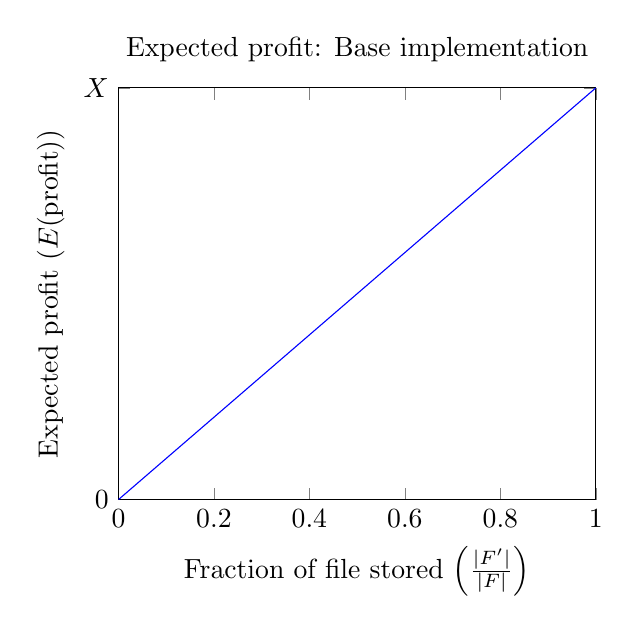
\begin{tikzpicture}
  \begin{axis}[ 
    xmin=0, xmax=1,
    ymin=0, ymax=1,
    xlabel={Fraction of file stored $\left(\frac{|F'|}{|F|}\right)$},
    ylabel={Expected profit ($E(\text{profit})$)},
    ytick={0,1},
    yticklabels={0, $X$},
    domain=0:1,
    title={Expected profit: Base implementation},
    scale only axis,
    width=0.5\textwidth,
  ]
    \addplot[color=blue,mark={}]{x}; 
  \end{axis}
\end{tikzpicture}

\caption[Expected attacker profit: base implementation]{Expected profit against proportion of chunks stored by node for the base contract implementation.}
\end{figure}


\subsection{Multiple chunk proofs}

See section \ref{multi-chunk} for details.

Here we require $c$ valid Merkle tree proofs for different chunks.
I assume that the chunks are chosen with replacement as this is how I have implemented it.
\[E(\text{profit}) = X \cdot \left(\frac{|F'|}{|F|}\right)^c\]

As can be seen in Figure~\ref{fig:eval-graph-multi} this makes it more profitable to store the whole file rather than a subset of the chunks.
Larger values of $c$ give more aggressive curves, but increase the size of the proof and therefore the transaction costs.


\begin{figure}[H] %**
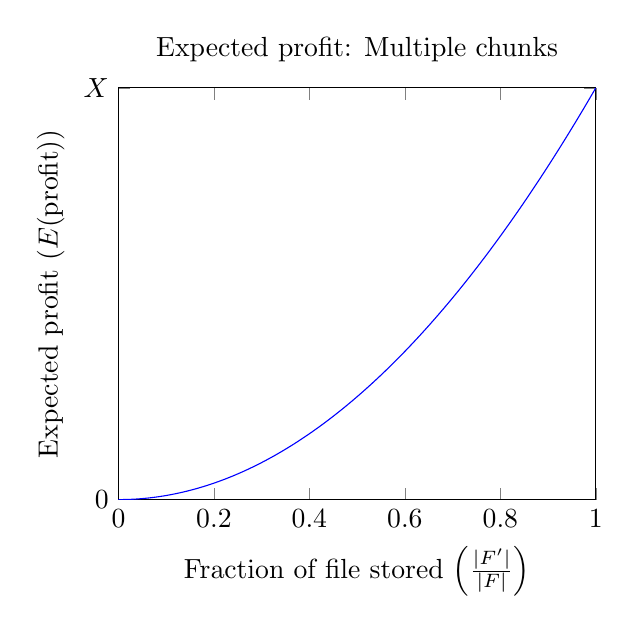
\begin{tikzpicture}
  \begin{axis}[ 
    xmin=0, xmax=1,
    ymin=0, ymax=1,
    xlabel={Fraction of file stored $\left(\frac{|F'|}{|F|}\right)$},
    ylabel={Expected profit ($E(\text{profit})$)},
    ytick={0,1},
    yticklabels={0, $X$},
    domain=0:1,
    samples=50,
    title={Expected profit: Multiple chunks},
    scale only axis,
    width=0.5\textwidth,
  ]
    \addplot[smooth,color=blue,mark={}]{x^2}; 
  \end{axis}
\end{tikzpicture}
\caption[Expected attacker profit: multiple chunk proofs]{Expected profit against proportion of chunks stored for the Multiple chunk proofs extension with $c = 2$.}
\label{fig:eval-graph-multi}
\end{figure}



%** * Do I need second graph
%\begin{figure}[H]
%\begin{tikzpicture}
%  \begin{axis}[ 
%    xmin=0, xmax=1,
%    ymin=0, ymax=1,
%    xlabel={Fraction of file stored $\left(\frac{|F'|}{|F|}\right)$},
%    ylabel={Expected profit per unit storage $\left(\frac{E(\text{profit})}{|F'|}\right)$},
%    ytick={0,1},
%    yticklabels={0, $\frac{X}{|F|}$},
%    domain=0:1,
%    samples=50,
%  ]
%    \addplot[smooth,color=blue,mark={}]{x}; 
%  \end{axis}
%\end{tikzpicture}
%\caption[Expected attacker profit per unit storage: multiple chunk proofs]{Expected profit per unit storage against proportion of chunks stored for the Multiple chunk proofs extension with $c = 2$.}
%\label{fig:eval-graph-multi-storage}
%\end{figure}

%*** \newpage
\subsection{Lock-in}

See section \ref{ext-lockin} for details.

Here the contract is given $X$ Ether by the owner and $L$ by the locking in storage node.
If the locking in storage node later submits a valid proof then they will receive the full $X + L$ as a reward.
\[E(\text{profit}) = (X + L) \cdot \frac{|F'|}{|F|} - L\]
Figure \ref{eval-graph-lockin} shows how this encourages nodes to store the whole file.

\begin{figure}[h]
\begin{tikzpicture}
  \begin{axis}[ 
    xmin=0, xmax=1,
    ymin=-2, ymax=1,
    xlabel={Fraction of file stored $\left(\frac{|F'|}{|F|}\right)$},
    ylabel={Expected profit ($E(\text{profit})$)},
    ytick={-2,0,1},
    yticklabels={$-L$, 0, $X$},
    axis lines=middle,
    x label style={at={(axis description cs:1.02,0.6666666)},anchor=west},
    ylabel near ticks,
    domain=0:1,
    scale only axis,
    width=0.5\textwidth,
    title={Expected profit: Lock in},
  ]
    \addplot[color=blue,mark={}]{3*x - 2}; 
  \end{axis}
\end{tikzpicture}
\caption[Expected attacker profit: lock-in]{Expected profit against proportion of chunks stored by node for the Lock-in extension with $L = 2X$.}
\label{eval-graph-lockin}
\end{figure}

%\begin{figure}[H]
%\begin{tikzpicture}
%  \begin{axis}[ 
%    xmin=0, xmax=1,
%    ymin=-2, ymax=1,
%    xlabel={Fraction of file stored $\left(\frac{|F'|}{|F|}\right)$},
%    ylabel={Expected profit per unit storage $\left(\frac{E(\text{profit})}{|F'|}\right)$},
%    ytick={-2,0,1},
%    yticklabels={$\frac{-L}{|F|}$, 0, $\frac{X}{|F|}$},
%    axis lines=middle,
%    x label style={at={(axis description cs:1.02,0.6666666)},anchor=west},
%    ylabel near ticks,
%    domain=0:1,
%  ]
%    \addplot[color=blue,mark={}]{(3*x - 2)/x}; 
%  \end{axis}
%\end{tikzpicture}
%\caption[Expected attacker profit per unit storage: lock-in]{Expected profit per unit storage against proportion of chunks stored by node for the Lock-in extension with $L = 2X$.}
%\label{eval-graph-lockin-storage}
%\end{figure}


\subsection{Erasure codes}

See section \ref{ext-erasure} for details.

Adding an Erasure code allows the file to be recovered even if some chunks are lost or corrupted.
For example, we could add 25\% to the file size to ensure that the file can be recovered even if 20\% (of the now larger file)
is lost.

Combining this with the other extensions in this section allows us to make it unprofitable to not store enough of the file to allow recovery,
as demonstrated in Figure~\ref{eval-graph-erasure}.
In this case a logical node will only ever lock in if they have space to store enough of the erasure encoded file for the
original to be recoverable.

Figure \ref{break-even-chunks} displays the fraction of the file that must be stored for a node to expect to break even
(and therefore the fraction that an erasure code should protect against losing)
against the number of chunks a proof is requested for.



\begin{figure}[h]
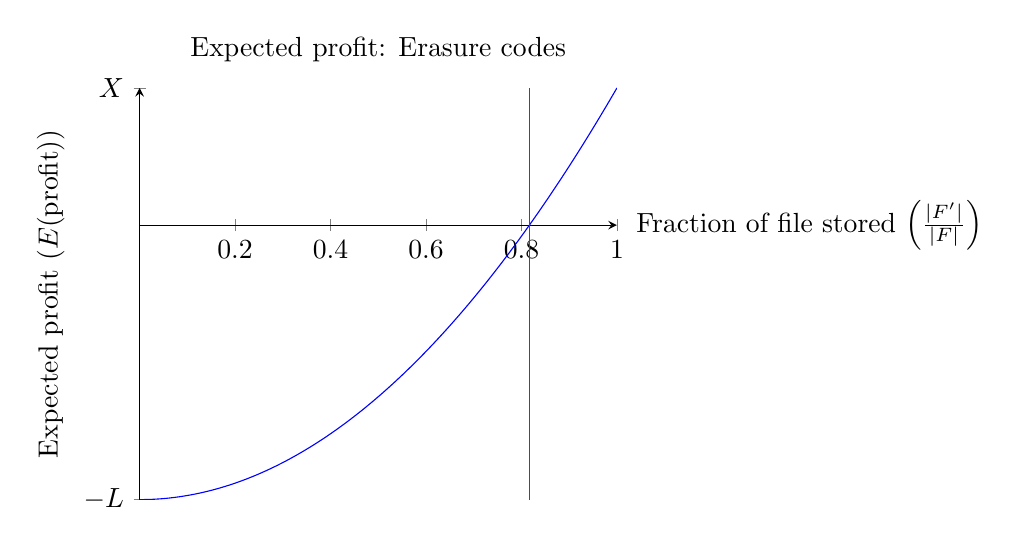
\begin{tikzpicture}
  \begin{axis}[ 
    xmin=0, xmax=1,
    ymin=-2, ymax=1,
    xlabel={Fraction of file stored $\left(\frac{|F'|}{|F|}\right)$},
    ylabel={Expected profit ($E(\text{profit})$)},
    ytick={-2,0,1},
    yticklabels={$-L$, 0, $X$},
    axis lines=middle,
    x label style={at={(axis description cs:1.02,0.6666666)},anchor=west},
    ylabel near ticks,
    domain=0:1,
    samples=50,
    scale only axis,
    width=0.5\textwidth,
    title={Expected profit: Erasure codes},
  ]
    \addplot[smooth,color=blue,mark={}]{3*x^2 - 2}; 
    \addplot[color=red,mark=none] coordinates {(0.816496580927726, -2) (0.816496580927726, 1)};
  \end{axis}
\end{tikzpicture}

\caption[Expected attacker profit: erasure code]{Expected profit against proportion of chunks stored with both the Lock-in extension and Multiple chunk proofs with $L = 2X$ and $c = 2$.
The red line represents the proportion ($\approx80\%$) of the chunks required to fully reconstruct the original file.}
\label{eval-graph-erasure}
\end{figure}

\FloatBarrier
\begin{figure}[h]
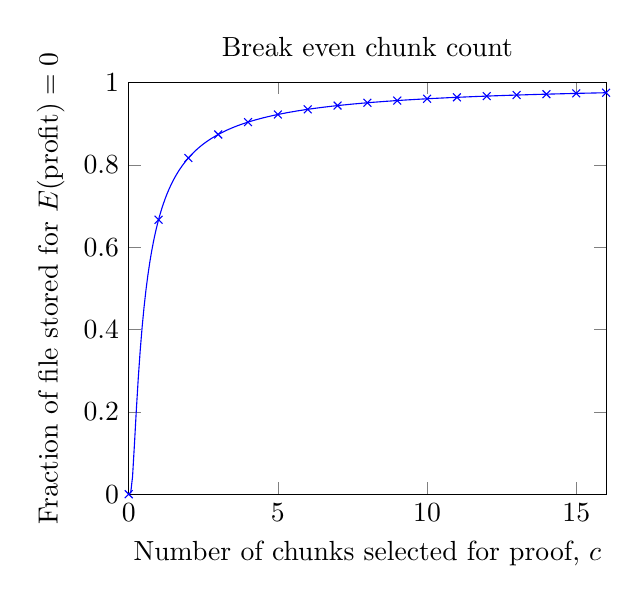
\begin{tikzpicture}
  \begin{axis}[ 
    xmin=0, xmax=16,
    ymin=0, ymax=1,
    xlabel={Number of chunks selected for proof, $c$},
    ylabel={Fraction of file stored for $E(\text{profit}) = 0$},
    domain=0:16,
    samples=250,
    title={Break even chunk count},
    scale only axis,
    width=0.5\textwidth,
  ]
    \addplot[color=blue,mark={}]{(2/3)^(1/x)};
    \addplot[color=blue, only marks, mark={x}, samples at={0.0001, 1, 2, 3, 4, 5, 6, 7, 8, 9, 10, 11, 12, 13, 14, 15, 16}]{(2/3)^(1/x)}; 
  \end{axis}
\end{tikzpicture}

\caption[Chunks to break even]{Fraction of $F$ that must be stored in order to have zero expected profit against the number of chunks required for the proof
when $L = 2X$ (see Appendix \ref{app-break-even-chunk-count} for details).} 
\label{break-even-chunks}
\end{figure}

\subsection{RSA extension}

The RSA extension behaves as a more efficient version of the Multiple chunk proofs extension.
This means we can increase the number of chunks the proof requires, making the profit curve much sharper.
For example, Figure \ref{eval-graph-RSA} demonstrates this with $c = 16$.

\begin{figure}[H]
\begin{tikzpicture}
  \begin{axis}[ 
    xmin=0, xmax=1,
    ymin=-2, ymax=1,
    xlabel={Fraction of file stored $\left(\frac{|F'|}{|F|}\right)$},
    ylabel={Expected profit ($E(\text{profit})$)},
    ytick={-2,0,1},
    yticklabels={$-L$, 0, $X$},
    axis lines=middle,
    x label style={at={(axis description cs:1.02,0.6666666)},anchor=west},
    ylabel near ticks,
    domain=0:1,
    samples=50,
    scale only axis,
    width=0.5\textwidth,
    title={Expected profit: RSA},
  ]
    \addplot[smooth,color=blue,mark={}]{3*x^16 - 2};
  \end{axis}
\end{tikzpicture}

\caption[Expected attacker profit: erasure code]{Expected profit against proportion of chunks stored with both the lock-in extension and multiple chunk proofs with $L = 2X$ and $c = 16$.
In this case it only becomes profitable when more than $97.5\%$ of the file is stored.}
\label{eval-graph-RSA}
\end{figure}
%*** Overveiw
%Was it successful, limitiations of Ethereum.

%\section{}

\chapter{Conclusion}

\section{Overview}
I have achieved my original aims for this project,
including a working implementation of the system described in my proposal and an analysis of its security and performance.
I have also completed several extensions and looked at the limitations of the Ethereum network with respect to this project.
I have demonstrated that it is practical to create an incentive system of this kind using Ethereum today;
the Evaluation chapter shows that my system is flexible and scales well with large files.

I am a little disappointed that I was unable to implement a secure RSA or ECC based Proof of Retrievability,
however my proof of concept worked well and it seems likely that a wholly secure implementation will be possible in the near future.

I have enjoyed completing the project and have learnt a lot about Ethereum and its ecosystem.
Whilst planning and implementing the RSA extension I also learnt more about modular arithmetic and group theory than I had
anticipated.

\section{Difficulties}
I encountered three main difficulties during the project:
\begin{itemize}
\item Learning about Ethereum

Ethereum is still young, and I found it was sometimes hard to find in depth information about some aspects of the protocol.
Similarly for Solidity, there was some good documentation, but it lacked detail.
I anticipated this to some extent going into the project however, so I had enough time to read around and understand what I needed to.

\item Understanding the literature on Proofs of Retrievability

Reading and understanding the papers I've seen on PoR took longer than I expected.
This was mostly due to my lack of background knowledge in areas such as elliptic curves, modular arithmetic
and group theory, which were used in the definitions and security proofs.

Between my reading around and the Security II course in Lent term of Part II
I've come to understand these areas enough to implement the RSA extension to my project.

\item Interoperating between Java and Solidity

I carefully planned out the interface between the contract and proof generator before I started implementation,
and because of this they worked together well.

I encountered more problems when testing the RSA extension.
This was partly due to the slightly different ways in which Java and Solidity handle big numbers,
as well as my lack of in-depth understanding as mentioned above.
These problems were exacerbated by the lack of tooling for Solidity, but I now have the RSA extension fully working with arbitrary files.
\end{itemize}

\section{Further work}

The next step that I would like to take, once the proposals for RSA and ECC pre-compiles have been deployed into Ethereum,
would be to write a fully secure Proof of Retrievability mechanism based on these primitives.
The RSA proof generation can already handle different modulus sizes and modifying the contract
should not be a huge undertaking, though multiplication for big numbers would need to be implemented as well
as the use of the pre-compiled contract for exponentiation.


Following on from that I would like to overlay this system onto an existing DFS, possibly as a fork of Swarm.






%%%%%%%%%%%%%%%%%%%%%
%Recent changes: Moved avoiding gas costs to appendix, modified the Swarm part to reflect that.
%Restructured end of prep (design) and start of impl (structure), moving the pseudo code from teh java bit of impl to the structure bit
%Restructured conclusion, mostly just adding sections

\begingroup
%\sloppy
\raggedright
\printbibliography
\endgroup

\begin{appendices}

\chapter{Proposal}


\includepdf[pages=-]{proposal.pdf}

\chapter{Contract code} \label{app-contract}

This is the source code for the contract with no extensions.
The all-caps constants (e.g. \texttt{PROOF\_LENGTH\_256\_BITS})
are replaced on a per-file basis by the Java code.

\lstinputlisting{partII_project/contract_final.sol}

\chapter{Java proof generation} \label{app-java}

This is the full Java code for the three functions described in pseudo-code in section \ref{pseudo-code}
for the root hash calculation, proof generation and proof verification.

\lstinputlisting{java_code.java}


\chapter{Configuration}

\section{Optimal chunk length} \label{app-chunk-size}

Recall section~\ref{chunk-size-proof-size}.
The size of a Merkle tree proof is:
\[|r| = C + 32 \cdot \left\lceil\log_2\left(\frac{|F|}{C}\right)\right\rceil\]
which can only be minimal when $\frac{|F|}{C}$ is a power of 2 (otherwise we can decrease $C$ and hence $|r|$ with no change in the log term).
Ignoring the ceil operation for a moment, the value of $c$ that minimises this will be $\frac{32}{ln(2)} \approx 46$.

We have $\frac{|F|}{C} = 2^n$ for some $n \in \mathbb{N}$, so we re-express $|r|$ in terms of $n$.
\[|r| = \frac{|F|}{2^n} + 32 n\]

We attempt to find the minimum, letting $n$ be in $\mathbb{R}$ for now.
\begin{align*}
\frac{d |r|}{d n} = 0 &\implies 32 - \ln(2) \cdot |F| \cdot 2^{-n} = 0\\
&\implies n = \log_2(|F|) - 5 + \log_2(\ln(2))
\end{align*}

An algorithm for computing the optimal chunk size follows from this
\begin{enumerate}
\item Compute the two natural numbers $n_1, n_2$ closest to $\log_2(|F|) - 5 + \log_2(\ln(2))$.
\item Let $C_i = \left\lceil \frac{|F|}{2^{n_i}}\right\rceil$.
\item Take $j \in \{1, 2\}$ such that $C_j + 32 \cdot \log\left(\frac{|F|}{C_j}\right)$ is minimized.
\item Return $C_j$.
\end{enumerate}

Because of the EVM's 32 byte word size, having a chunk size that is a multiple of 32 bytes simplifies the contract and results in lower gas costs
so I use 64 bytes as the chunk size by default.


\section{Break even chunk count}\label{app-break-even-chunk-count}

We wish to find the fraction of a file that must be stored when a proof for $c$ chunks is required in order to break even on average.
The contract reward is $X$ Ether with an $L$ Ether deposit required.

The chance that a storage node that keeps a fraction $\displaystyle \frac{|F'|}{|F|}$ of the $m$ chunk file can produce a proof for
$c$ randomly selected (with replacement) chunks is
$\displaystyle \left(\frac{|F'|}{|F|}\right)^c$.
Their expected profit is therefore
\[E(\text{profit}) = (X + L) \cdot \left(\frac{|F'|}{|F|}\right)^c - L\]
The node will break even when $E(\text{profit}) = 0$, in which case
\[\frac{|F'|}{|F|} = \left(\frac{L}{X+L}\right)^{1/c}\]

This gives the fraction of $F$ which should be protected by an erasure code in order for the system
to be secure against the threat models I gave in section \ref{threat-model}. %*** This is plotted in figure***






\chapter{Details on Ethereum}

\section{EVM storage}\label{evm-mem}

When executing, contracts have access to three types of memory:

\begin{itemize}
\item Stack

Intended for local variables, this is cheapest to access at 2 gas for a \texttt{POP} operation and 3 for a \texttt{PUSH}\footnote{All gas values are taken from the
12-04-2017 revision of the Ethereum Yellow Paper\cite{eth-yellowpaper}.}.
It does not persist between calls to the contract.

\item Memory

Analogous to the a heap in a normal execution environment, larger structures and arrays can be stored here.
It is very slightly more expensive to access than the stack at 3 gas for a load operation and the same for a store.
It does not persist between calls to the contract.

\item Storage

Permanent storage on the blockchain, allowing data to persist between contract invocations.
In comparison this is extremely expensive.
A load is 50 gas, a write to an existing location is 5000 gas and writing to a new word of storage costs 20000 gas.
\end{itemize}

Sending a 1kb file to a contract costs about 2.25 million gas (found empirically by sending 1kb of random data to a test contract)
or about \textsterling1.40.
Storing 1kb of data costs an additional 64000 gas.
This might be useful as a way to replicate small but valuable files, but at over \textsterling1000 per megabyte
storing large files on the blockchain is clearly impractical.

Gas costs are taken from the Ethereum Yellow Paper\cite{eth-yellowpaper}.


\section{Uncle blocks}\label{app-uncle}

If a miner generates a valid block, but is too slow to distribute it to the network then a different miner may
have their block accepted instead and take the block reward.
Ethereum has a much lower block time than Bitcoin (14 seconds instead of 10 minutes) so wasted miner time is a significant problem.
To counter this Ethereum allows stale blocks to be mentioned later in the chain as `Uncles'.

When this happens the block header of the Uncle block is included as part of a main chain block, giving the miner of the Uncle block a reduced reward,
starting at $\frac{7}{8}$ of the normal 5 Ether reward.
The Uncle reward is reduced by a further $\frac{1}{8}$ of the normal block reward for each
block behind the current one the Uncle is the sibling of, down to a minimum of $\frac{2}{8}$ after 6 blocks
at which point it is no longer valid to mention an Uncle.
Only two Uncle blocks can be mentioned per main block.
The node that mines the block which mentions the Uncle also gets an extra $\frac{1}{32}$ of the normal reward.
Full detail on the Uncle system is available in the Ethereum Yellow Paper\cite{eth-yellowpaper}.





\chapter{Contract structure}\label{app-challenge}

It is possible to structure a contract such that the proof verification algorithm only needs to be run if the file owner issues a challenge to the storing node,
thus saving on transaction costs.
The content of this section is something I considered when I was designing and building the contract, and is relevant to contract design, but it is not important for
understand the rest of the report so I have placed it in the Appendix:

For this section I will assume the lock-in extension is used and a storing node must provide a deposit as a promise they will keep their file.

So far in my discussions I have assumed there is no interaction from the file owner once the contract has been deployed
and the storing node must always provide a proof to claim the reward:
\begin{itemize}
\item The storing node sends a transaction to the contract with Ether for a deposit.
The contract records the address the transaction comes from on the blockchain.

\item Later the storing node sends a Proof of Retrievability to the contract.
The contract checks that the address of the sender matches the one it has stored as well as verifying the proof
before paying out.
\end{itemize}

This format is demonstrated by Figure \ref{project-overview} from the Introduction.
This design is sensible for my Merkle tree contract because the gas costs for verification are generally quite low (70777 gas or about five pence for an 8MB file),
that said it would be reasonably simple to modify my contract to use a challenge system for proofs.
For a different PoR system, like in my RSA extension or for Swarm it can make more sense to use a challenge based system.




\subsubsection{Challenge system}

The contract can be redesigned so that a proof is only required if the file owner believes that the
storage node does not have the file. The idea is the storing node will show the file owner a proof off-chain,
thus resulting in lower transaction costs without losing any security.
This is shown in Figure \ref{fig-challenge}.

\begin{itemize}
\item The storing node sends a deposit to the contract in the same way as before.

\item By default the storing node will be able to collect the reward after some time without providing a proof.

\item The file owner may issue a challenge by providing the contract with a small Ether deposit.

\item If the storing node responds to the challenge with a correct proof they are given all the funds in the contract.

\item If the storing node fails to provide a proof within some time limit then the file owner recovers 
the funds from the contract.
\end{itemize}

This version has the advantage that the proof verification algorithm
does not need to be run if a challenge is never made, thus saving on gas costs,
however it requires more involvement from the file owner.
The challenge deposit should be less than the gas cost of proof verification
which encourages the storing node to provide a proof to the owner privately off-chain,
but still enough to discourage unnecessary challenges.

\begin{figure}[H]
\centering
\hspace*{-0.8cm}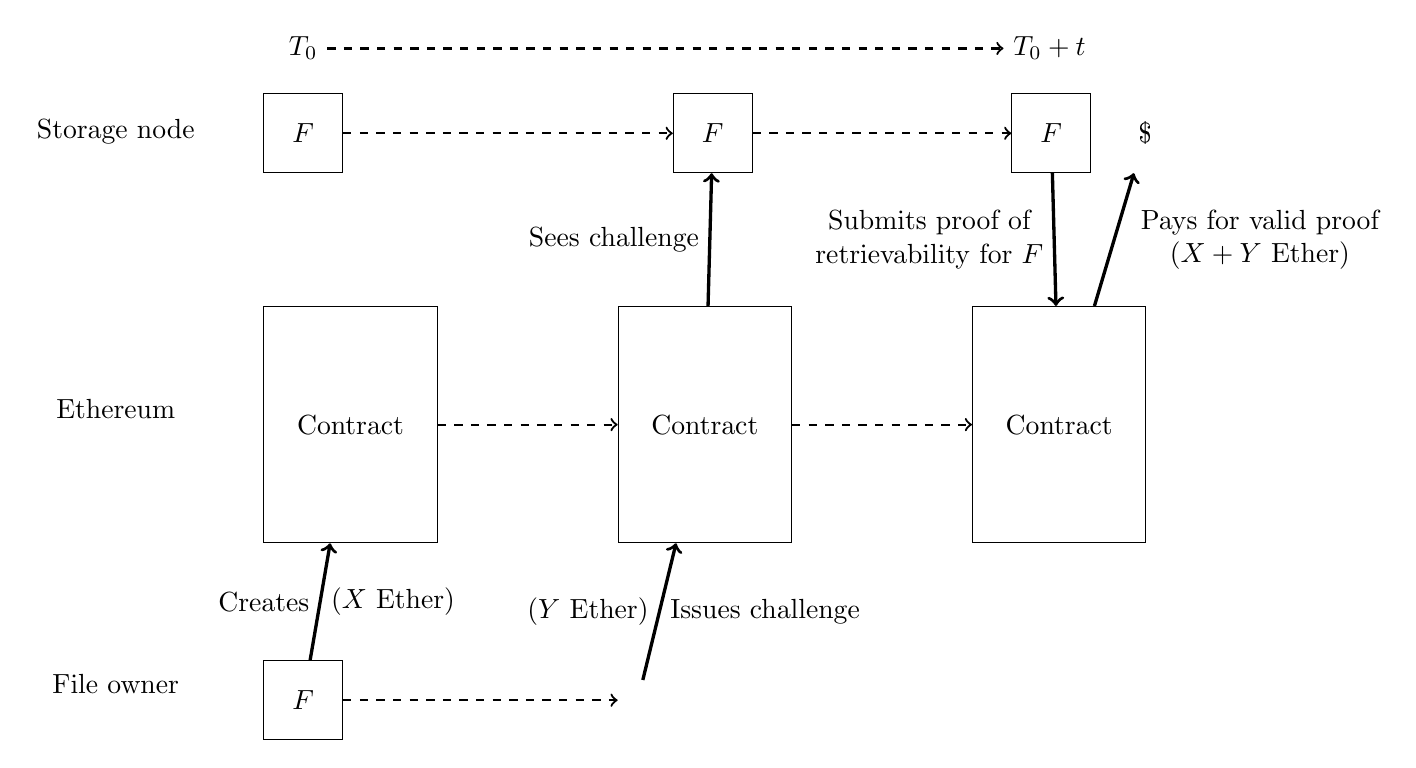
\begin{tikzpicture}


\coordinate(O1) at (0,0);
\node[above right=0.5cm and 3.2cm of O1](t0) {$T_0$};
\node[above right=0.5cm and 12.4cm of O1](t1) {$T_0 + t$};

\node[below right=0cm of O1](s) {Storage node};
\node[below = 3 cm of s](b) {Ethereum};
\node[below = 3 cm of b](o) {File owner};

\node[below right=-0.2cm and 3cm of O1,draw, minimum width=1cm,minimum height=1cm,fill=white](sf) {$F$};
\node[below right=7cm and 3cm of O1,draw, minimum width=1cm,minimum height=1cm,fill=white](of) {$F$};

\node[below right=2.5cm and 3cm of O1,draw, minimum width=2.2cm,minimum height=3cm,fill=white](c) {Contract};

\node[below right=2.5cm and 7.5cm of O1,draw, minimum width=2.2cm,minimum height=3cm,fill=white](cm) {Contract};
\node[below right=-0.2cm and 8.2cm of O1,draw, minimum width=1cm,minimum height=1cm,fill=white](sfm) {$F$};
\node[below right=7.25cm and 7.5cm of O1,minimum width=0.5cm,minimum height=0.5cm](ofm) {};

\node[below right=-0.2cm and 12.5cm of O1,draw, minimum width=1cm,minimum height=1cm,fill=white](sft) {$F$};
\node[below right=2.5cm and 12cm of O1,draw, minimum width=2.2cm,minimum height=3cm,fill=white](ct) {Contract};
\node[below right=-0.2cm and 13.7cm of O1,minimum width=1cm,minimum height=1cm,fill=white](smoneyt) {\$};


\draw[->, very thick] (of) -- node[left] {Creates} node[right] {($X$ Ether)} (c);
\draw[->, thick, dashed] (t0) -- (t1);
\draw[->, thick, dashed] (c) -- (cm);
\draw[->, thick, dashed] (cm) -- (ct);
\draw[->, thick, dashed] (sf) -- (sfm);
\draw[->, thick, dashed] (sfm) -- (sft);
\draw[->, very thick] (sft) -- node[left, align=center] {Submits proof of\\ retrievability for $F$} (ct);
\draw[->, very thick] (ct) -- node[right=0.2cm, align=center] {Pays for valid proof\\($X+Y$ Ether)} (smoneyt);
\draw[->, very thick] (ofm) -- node[right] {Issues challenge} node[left] {($Y$ Ether)} (cm);
\draw[->, very thick] (cm) -- node[left] {Sees challenge} (sfm);
\draw[->, thick, dashed] (of) -- (ofm);
\end{tikzpicture}
\caption[Project overview]{An overview of the proposed structure of the project.}
\label{fig-challenge}
\end{figure}


\subsubsection{Report liar}

If the cost of verifying the proof is significantly larger than the cost of just uploading it then
it can be sensible to always upload the proof, but not immediately verify it.
The storage node (or anyone, depending on the design) may then report the storing node as a liar by calling a different function on the contract
and providing enough gas to run the verification function.
Users can run the verification algorithm off-chain before deciding whether to issue a challenge.

\subsubsection{Receipt}

The aim here is to keep as little state as possible in the case of a generic contract handling multiple files, owners and storage nodes.
Any storage node wishing to sell receipts must send a security deposit to the contract.
The file owner buys a signed receipt off a storage node containing some information about the file and an expiry time.
To make a challenge the file owner presents the receipt to the contract at which point the storing node is required to upload a valid proof
or lose their deposit. Swarm intends to use a receipt based system.







%\chapter{Block hash as a random number} \label{app-block-hash}
%
%This is more complete analysis of the question raised in section \ref{sec-block-hash} of whether the block hash of
%some block is suitable as a random number.
%I want to look at how much of an advantage a storing node would have in my system if they control a significant proportion of the mining power.
%%I will assume that the miner or colluding miners in question have at most $40\%$ of the total mining power, keeping in mind that more that $50\%$
%%gives them complete control of the network.
%
%\section{Uncle blocks}
%
%Ethereum has a much lower block time than Bitcoin (fourteen seconds versus 10 minutes).
%This is a problem because it discourages the inclusion of transactions in blocks.
%People sending transactions include a small transaction fee which is collected by the miner, giving an incentive for
%them to include transactions in blocks.
%However the more transactions are included in a block the longer it will take to process and distribute through the network,
%thus increasing the chances that some other miner will produce the block first, meaning loss of the block reward.
%This means that transaction fees must be much higher to compensate for the possibility of losing the block reward.
%
%To counteract this Ethereum has a concept of uncle blocks, stale blocks that were too slow to be accepted as the next block in the chain,
%but still eligible for a reduced block reward (though not any transaction fees).
%This means that even if a miner is too slow propagating their block they can still collect a reduced reward
%and therefore are more likely to include transactions.
%The uncle blocks also add `weight' to the chain (and the `heaviest' is considered to be correct),
%reducing wasted hash power and increasing the network's security.
%%The Ethereum White Paper\cite{eth-whitepaper} and the Homestead release documentation\cite{eth-homestead}
%%have more details.
%
%\subsection{Details of the Uncle block protocol}
%
%Full detail is given in the Ethereum Yellow Paper\cite{eth-yellowpaper},
%which I draw this information from.
%
%A block may mention at most two uncles,
%and they must be siblings of one of the last six blocks, not including the current one, giving a total of twelve uncle slots for a
%given generation assuming they are not taken by other generations.
%The miner of the block gets an extra $\frac{1}{32}$ of the block reward for each uncle mentioned.
%The miner of each uncle gets the block reward reduced by $\frac{1}{8}$ for each block distant
%from the current one that the uncle is a sibling of, meaning at most a reward of $\frac{7}{8}$ of the normal block reward
%and at least $\frac{2}{8}$ of the normal reward.
%
%\section{Manipulating the block hash}
%
%Consider a storing node that is also a miner.
%They have not stored the whole of the file that the contract is for
%and only have a chance $q$ of being able to generate a valid proof for a random key $\kappa$ and claim the $X$ Ether (here $X$ includes the lock in deposit if one exists).
%Suppose that this node mines block $T_0 + t$, on which $\kappa$ depends, and finds that they cannot generate a valid proof for the contract
%if this block is accepted by the network.
%The node could keep the block private and submit it later as an uncle, claiming the reduced reward.
%They would then get to `re-roll' the block hash, getting another $q$ chance to be able to generate a valid proof.
%I will assume that this nodes Uncle blocks are included as soon as possible in the chain and ignore lost transaction fees.
%I'll also assume that by publishing the block the node will always be first and can collect the full block reward.
%
%\subsection{When is it worth it for a node to not publish a block?}
%
%A node that has a negligible fraction of the mining power will keep a block with a bad hash private if 
%\[q \cdot X > U_L\]
%where $U_L$ is the loss from only creating an uncle block, $\frac{5}{8}$ Ether.
%
%If a node controls a non-negligible fraction $p$ of the mining power then there is a chance they will generate the next block
%too and get another chance to re-roll.







\end{appendices}
\end{document}
